%%%%%%%%%%%%%%%%%%%%%%%%%%%%%%%%%%%%%%%%%
% Short Sectioned Assignment
% LaTeX Template
% Version 1.0 (5/5/12)
%
% This template has been downloaded from:
% http://www.LaTeXTemplates.com
%
% Original author:
% Frits Wenneker (http://www.howtotex.com)
%
% License:
% CC BY-NC-SA 3.0 (http://creativecommons.org/licenses/by-nc-sa/3.0/)
%
%%%%%%%%%%%%%%%%%%%%%%%%%%%%%%%%%%%%%%%%%

%----------------------------------------------------------------------------------------
%	PACKAGES AND OTHER DOCUMENT CONFIGURATIONS
%----------------------------------------------------------------------------------------

\documentclass[paper=a4, fontsize=11pt]{scrartcl} % A4 paper and 11pt font size

\usepackage[T1]{fontenc} % Use 8-bit encoding that has 256 glyphs
%\usepackage[ngerman]{babel}
\usepackage{fourier} % Use the Adobe Utopia font for the document - comment this line to return to the LaTeX default
\usepackage{amsmath,amsfonts,amsthm} % Math packages
\usepackage{graphicx}
\usepackage[utf8]{inputenc}
\usepackage{listings}
\usepackage[section]{placeins}
\usepackage{lipsum} % Used for inserting dummy 'Lorem ipsum' text into the template
\usepackage{float}
\usepackage{multicol}
\usepackage{varwidth}
\usepackage{sectsty} % Allows customizing section commands
\usepackage{enumitem}
\allsectionsfont{\centering \normalfont\scshape} % Make all sections centered, the default font and small caps

\usepackage{fancyhdr} % Custom headers and footers
\pagestyle{fancyplain} % Makes all pages in the document conform to the custom headers and footers
\fancyhead{} % No page header - if you want one, create it in the same way as the footers below
\fancyfoot[L]{} % Empty left footer
\fancyfoot[C]{} % Empty center footer
\fancyfoot[R]{\thepage} % Page numbering for right footer
\renewcommand{\headrulewidth}{0pt} % Remove header underlines
\renewcommand{\footrulewidth}{0pt} % Remove footer underlines
\setlength{\headheight}{13.6pt} % Customize the height of the header

\numberwithin{equation}{section} % Number equations within sections (i.e. 1.1, 1.2, 2.1, 2.2 instead of 1, 2, 3, 4)
\numberwithin{figure}{section} % Number figures within sections (i.e. 1.1, 1.2, 2.1, 2.2 instead of 1, 2, 3, 4)
\numberwithin{table}{section} % Number tables within sections (i.e. 1.1, 1.2, 2.1, 2.2 instead of 1, 2, 3, 4)

\setlength\parindent{0pt} % Removes all indentation from paragraphs - comment this line for an assignment with lots of text

\DeclareMathOperator*{\argmin}{arg\,min}
\DeclareMathOperator*{\argmax}{arg\,max}

%----------------------------------------------------------------------------------------
%	TITLE SECTION
%----------------------------------------------------------------------------------------

\newcommand{\horrule}[1]{\rule{\linewidth}{#1}} % Create horizontal rule command with 1 argument of height

\title{	
\normalfont \normalsize 
\textsc{Karlsruhe Institute of Technology} \\ [25pt] % Your university, school and/or department name(s)
\horrule{0.5pt} \\[0.4cm] % Thin top horizontal rule
\huge Accessibility - Assistive Technologies for Visually Impaired Persons % The assignment title
\horrule{2pt} \\[0.5cm] % Thick bottom horizontal rule
}

\author{Manuel Lang} % Your name

\date{\normalsize\today} % Today's date or a custom date

\begin{document}

\maketitle % Print the title
\newpage
\tableofcontents
\newpage

\section{Einführung}

\begin{itemize}
\item Weltweit ca. 285 Millionen Sehbehinderte (über 39 Millionen Blinde)
\item In Deutschland 500.000 bis 1.1 Millionen Sehbehinderte (160.000 Blinde)
\item Verlust des Sehvermögens bringt Einschränkungen in Mobilität, Kommunikation, Zugang zu Informationen, Kognitive Aktivitäten, Alltag, Ausbildung und Arbeitstag, Freizeitaktivitäten, ...
\item Mit Assistiven Technologien (AT) können viele Dinge nicht behoben, aber wesentlich vereinfacht werden
\end{itemize}

\section{Hilfsmittel im Alltag}

\subsection{Hilfsmittel im Haushalt}

\begin{minipage}[c]{0.55\textwidth}
\begin{itemize}
\item Wäschepflege: Farberkennung, Sortierung, Waschmitteldosierung
\item Kennzeichnung
\item Bsp.: Etikettenlesegerät, Farberkenner
\end{itemize}
\end{minipage}
\begin{minipage}[c]{0.3\textwidth}
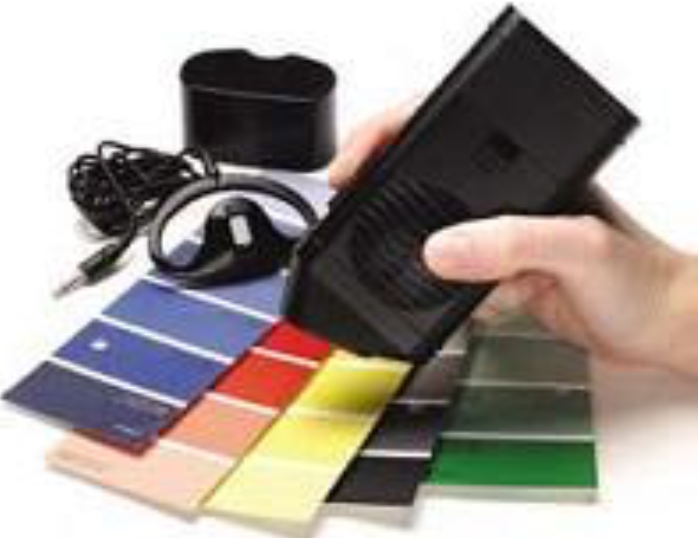
\includegraphics[width=\textwidth]{imgs/farbleser}
\end{minipage}

\subsection{Messen und Wahrnehmen}

\begin{minipage}[c]{0.55\textwidth}
\begin{itemize}
\item Gewichte, Längen, Temperatur, Licht, Wetter
\item Bsp.: Sprechendes Maßband, Lichtdetektor, Messkoffer
\end{itemize}
\end{minipage}
\begin{minipage}[c]{0.3\textwidth}
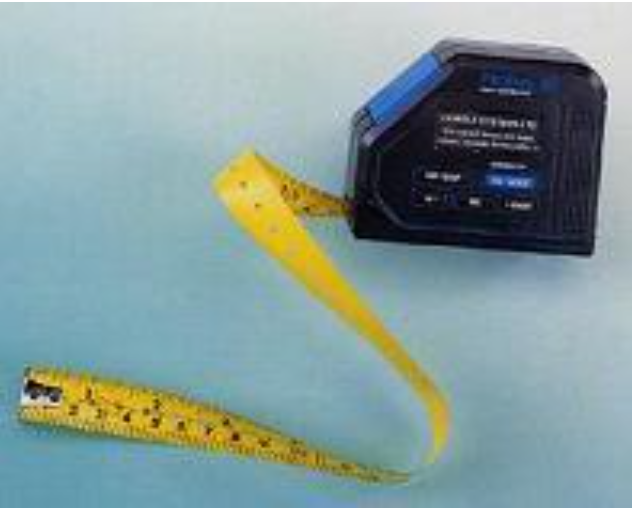
\includegraphics[width=\textwidth]{imgs/massband}
\end{minipage}

\subsection{Schreiben, Lesen, Rechnen}

\begin{minipage}[c]{0.55\textwidth}
\begin{itemize}
\item Punktschrift-Schreibmaschine
\item Punktschrifttafel
\item Abakus
\item Rechenkasten
\item sprechender Taschenrechner
\end{itemize}
\end{minipage}
\begin{minipage}[c]{0.3\textwidth}
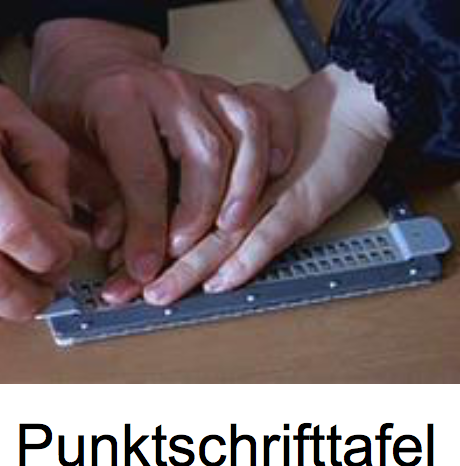
\includegraphics[width=\textwidth]{imgs/punktschrift}
\end{minipage}

\subsection{Information und Multimedia}

\begin{minipage}[c]{0.55\textwidth}
\begin{itemize}
\item Diktiergerät
\item Daisy-Player
\item Computer
\item Braillezeile
\item Sprachausgabe
\item Smartphone
\end{itemize}
\end{minipage}
\begin{minipage}[c]{0.35\textwidth}
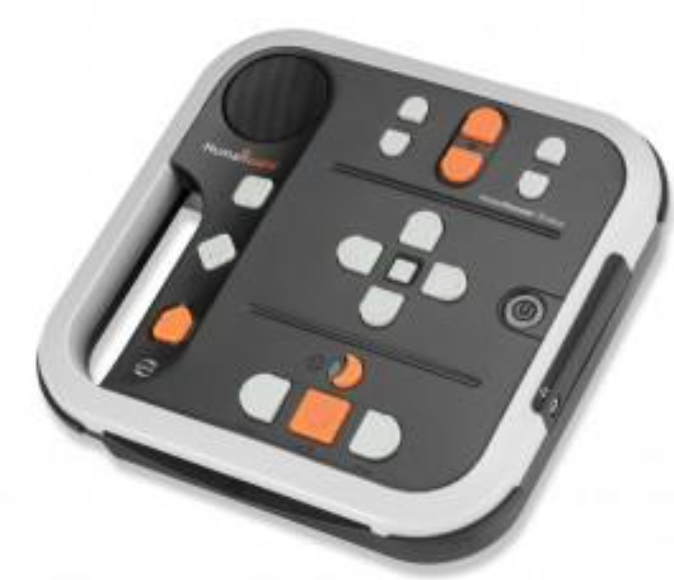
\includegraphics[width=\textwidth]{imgs/daisy}
\end{minipage}

\subsection{Erkennen und Verstehen}

\begin{minipage}[c]{0.55\textwidth}
\begin{itemize}
\item Texterkennung, Objekterkennung
\item Kommunikation mit Ton und Bild: Twitter, Face Time, Skype, Siri
\end{itemize}
\end{minipage}
\begin{minipage}[c]{0.35\textwidth}
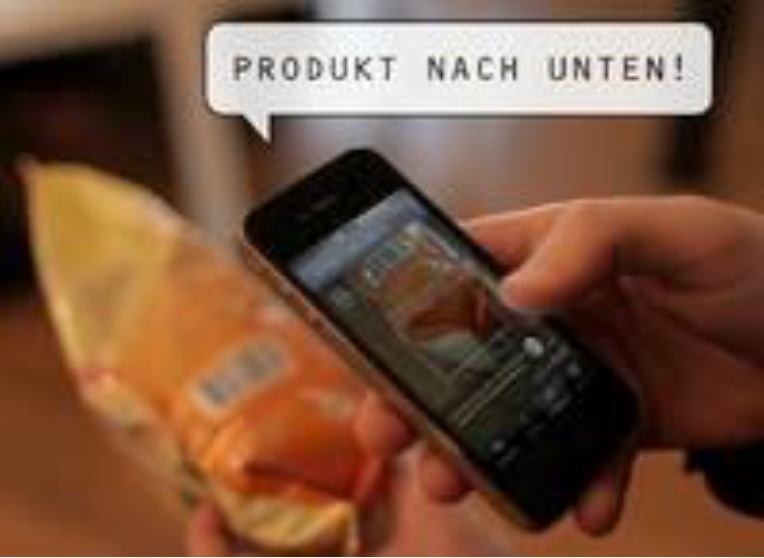
\includegraphics[width=\textwidth]{imgs/iphone}
\end{minipage}

\subsection{Mobilität und Orientierung}

\begin{minipage}[c]{0.55\textwidth}
\begin{itemize}
\item Langstock
\item Clicksonar
\item Hinderniserkennung
\item Entfernungsbestimmung
\item Navigation (Kompass)
\end{itemize}
\end{minipage}
\begin{minipage}[c]{0.35\textwidth}
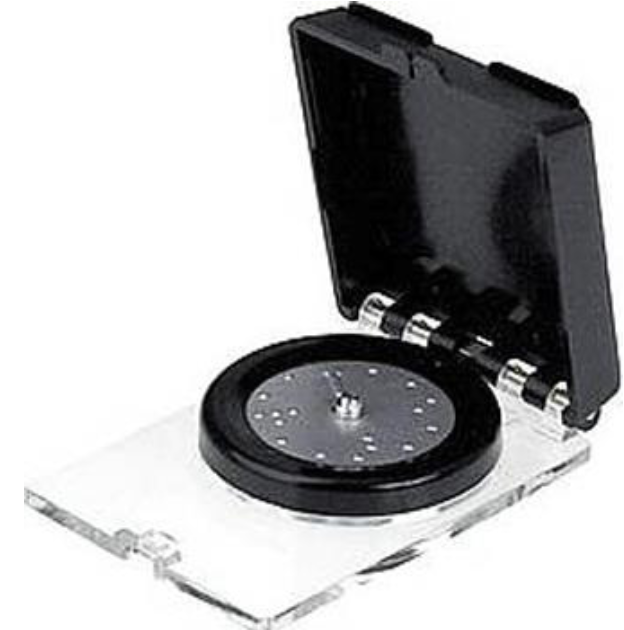
\includegraphics[width=\textwidth]{imgs/kompass}
\end{minipage}

\subsection{Teilhabe durch Technologie}

\begin{itemize}
\item Zugang zu Bildung und Wissen
\item Internet, Ebooks, Podcasts, Epaper etc.
\item Früher: Kassettenaufsprache, gekürzte Zeitungen, eingeschränkte Auswahl
\item Bewusst zensiert und Vorenthalt von Informationen, die für Bilde moralisch schädlich sind (Zugang zu Tabuthemen)
\end{itemize}

\subsection{Ausblick}

\begin{itemize}
\item Verbesserung der Genauigkeit bei der Navigation durch Galileo
\item Entwicklung Indoor-Navigation
\item Unterstützung in Orientierung \& Mobilität durch kamerabasierte Hilfsmittel
\item Kombination von GPS, Kartendatenbank, Maschinensehen, RFID, etc.
\item Trends
\begin{itemize}
\item Immer mehr Touchscreens
\begin{itemize}
\item Steuerung von Haushaltsgeräten (Spülmaschine, Kaffeemaschine)
\item Öffentliche Automaten (Geldautomat, Snackautomat)
\item Technologien für taktile Displays
\item Standardisierung von einheitlichen Schnittstellen zu AT
\end{itemize}
\item Assistenzroboter
\begin{itemize}
\item Unterstützung im Haushalt (Putzen, Staubsaugen)
\item Orientierung und Mobilität (elektronischer Blindenführhund, Einkaufhilfe)
\item Interaktion- und Kommunikationsfähigkeit (Sprachsteuerung)
\end{itemize}
\item Smart-Home-Steuerung
\begin{itemize}
\item Überwachung von Geräte-Status (Herd Ein/Aus)
\item Lichtkontrolle
\item Zugang zu Stromzähler
\item Temperatursteuerung
\end{itemize}
\item Einsatz von Weables
\begin{itemize}
\item Interaktion mit AT und Umwelt
\item Zusätzlicher Informationskanal (Hindernisanzeige durch Vibration)
\item Entlastung des Audiokanals
\item Diskrete Erweiterung der AT (Navigation)
\end{itemize}
\item IoT
\begin{itemize}
\item Schnittstelle zu unbedienbaren Geräten (Fernseher, Haushaltsgeräte)
\item Erhöhung der Sicherheit (Rauchmelder)
\item Statusmeldungen (Was ist noch im Kühlschrank?)
\end{itemize}
\item Lernfähige Systeme
\begin{itemize}
\item Objekterkennung (Computer Vision)
\item Adaption der Hilfstechnologie an Nutzer
\item Potential zur Verbesserung Orientierung und Mobilität
\end{itemize}
\end{itemize}
\end{itemize}

\section{Grundlagen}

\subsection{Integration/Inklusion}

\begin{minipage}[c]{0.55\textwidth}
\begin{itemize}
\item Integration: Engliederung von Menschen mit Behinderungen in die bestehende Gesellschaft
\item Inklusion: selbstverständliche Berücksichtigung der Bedürfnisse aller Mitglieder der Gesellschaft, Verschiedenheit aller Menschen, Vielfalt = Diversität/Diversity, Heterogenität als Normalität
\end{itemize}
\end{minipage}
\begin{minipage}[c]{0.35\textwidth}
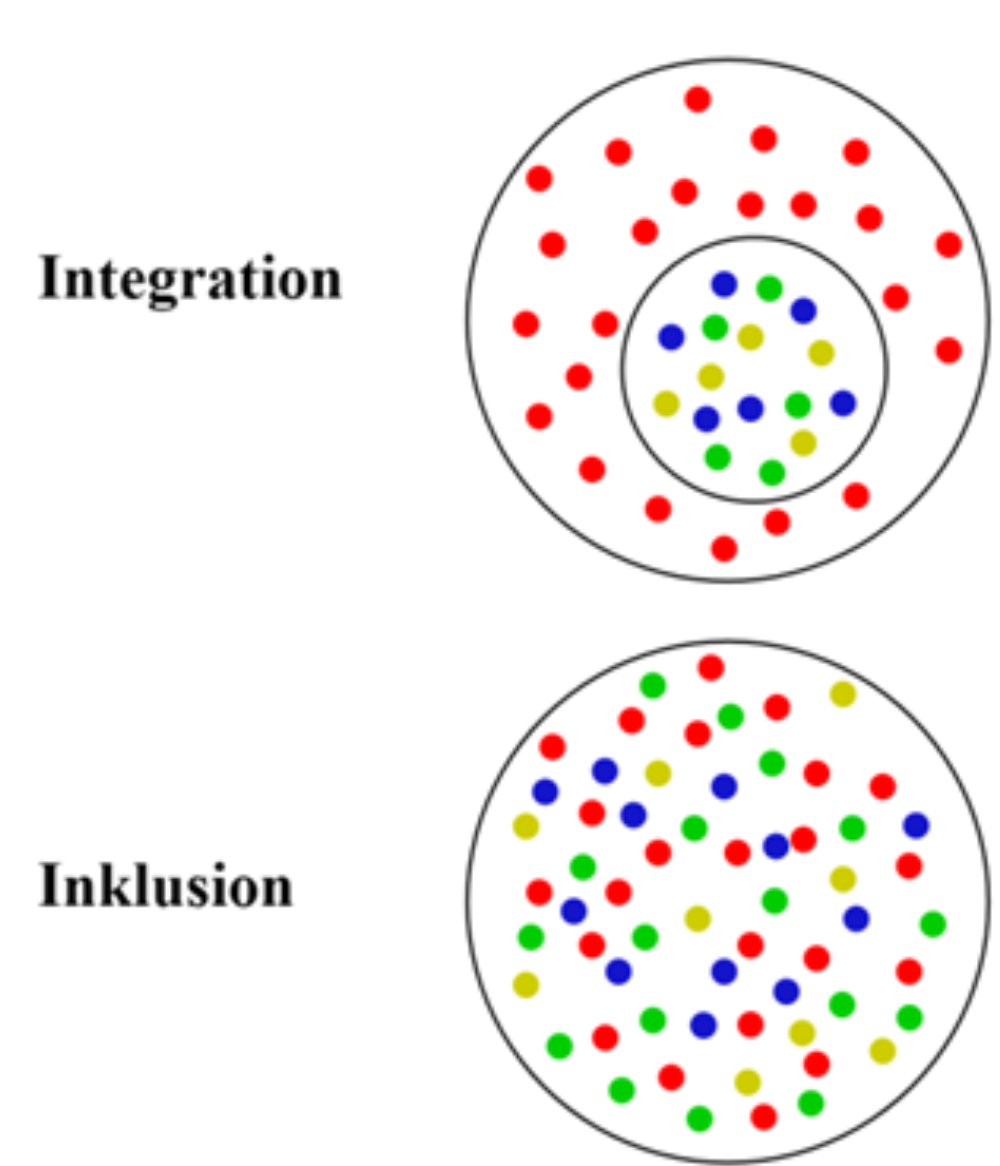
\includegraphics[width=\textwidth]{imgs/inklusion}
\end{minipage}

\subsection{Konventionen}

\begin{itemize}
\item \textbf{UN-BRK Behindertenrechtskonvention}: ``Zu den Menschen mit Behinderungen zählen Menschen, die langfristige körperliche, sellische, geistige oder andere Sinnesbeeinträchtigungen haben, welche sie in Wechselwirkung mit verschiedenen Barrierefreien an der vollen, wirksamen und gleichberechtigten Teilhabe an der Gesellschaft hindern können.''
\item Wandlung vom medizinischen zum gesellschaftlichen Modell: Behinderung/chronische Krankheit liegt nicht im Menschen begründet, sondern die Gesellschaft/Umwelt behindert.
\item \textbf{BGG Behindertengleichstellungsgesetz und SGB Sozialgesetzbuch IX}: §2 (1) ``Menschen sind behindert, wenn ihre körperliche Funktion, geistige Fähigkeit oder seelische Gesundheit mit hoher Wahrscheinlichkeit länger als sechs Monate von dem für das Lebensalter typischen Zustand abweichen und daher ihre Teilhabe am Leben in der Gesellschaft beeinträchtigt ist.''
\item \textbf{GG Grundgesetz}: §3 (3) ``Niemand darf wegen seinen Geschlechtes, seiner Abstammung, seiner Rasse, seiner Sprache, seiner Heimat und Herkunft, seines Glaubens, seiner religiösen oder politischen Anschauung benachteiligt oder bevorzugt werden. \textbf{Niemand darf wegen seiner Behinderung benachteilig werden.}''
\item Definitionen zu Blindheit und Sehbehinderung unterscheiden sich zwischen gesetzlicher Definition und WHO-Definition
\begin{itemize}
\item Gesetz spricht bei unter 2\% von Blindheit, WHO bei unter 5\%
\item Gesetzlich werden Leute mit 2\% - 5\% als hochgradig sehbehindert bezeichnet
\item Sehbehinderung bei 5\% - 30\%
\end{itemize}
\item Ursachen: angeboren, Unfall (Durchtrennung des Sehnervs, ...), Alter, Krankheit (Schlaganfall, Tumor, ...)
\item Sehbehinderungen: Grauer Star, Grüner Star, Makuladegeneration, Diabetische Retinopathie, Retinitis Pigmentosa, Netzhautablösung, Albinismus, Achromatopsie (Farbenblindheit) ...
\end{itemize}

\subsection{Braille (Arten, Versionen, Speziallösungen)}

\begin{itemize}
\item Von hinten in Papier gepresstes, mit Fingerkippen ertastbares Punktmuster, Punktekombinationen
\item Bis Einführung Computer 6-Punkt-Schrit (Würfel), drei Pixel in Höhe, zwei in Breite, 6mm lang, 4mm breit, Punkthöhe > 0,4mm
\item Braille kann als das erste binäre System gesehen werden.
\item Zählung absteigend linke Spalte 1 bis 3, rechte 4 bis 6 (Computerbraille/8-Punkt Braille: 7 und 8 unterhalb)
\item Die Punkte sind in keiner offensichtlichen Reihenfolge angeordnet
\item Seit 1992 ist 8-Punkt Schrift (= Computerbraille) Standard, da 6-Punkt-Schrift nur $2^6 = 64$ mögliche Belegungen bietet und somit Doppelbelegungen unausweichlich sind.\\ 
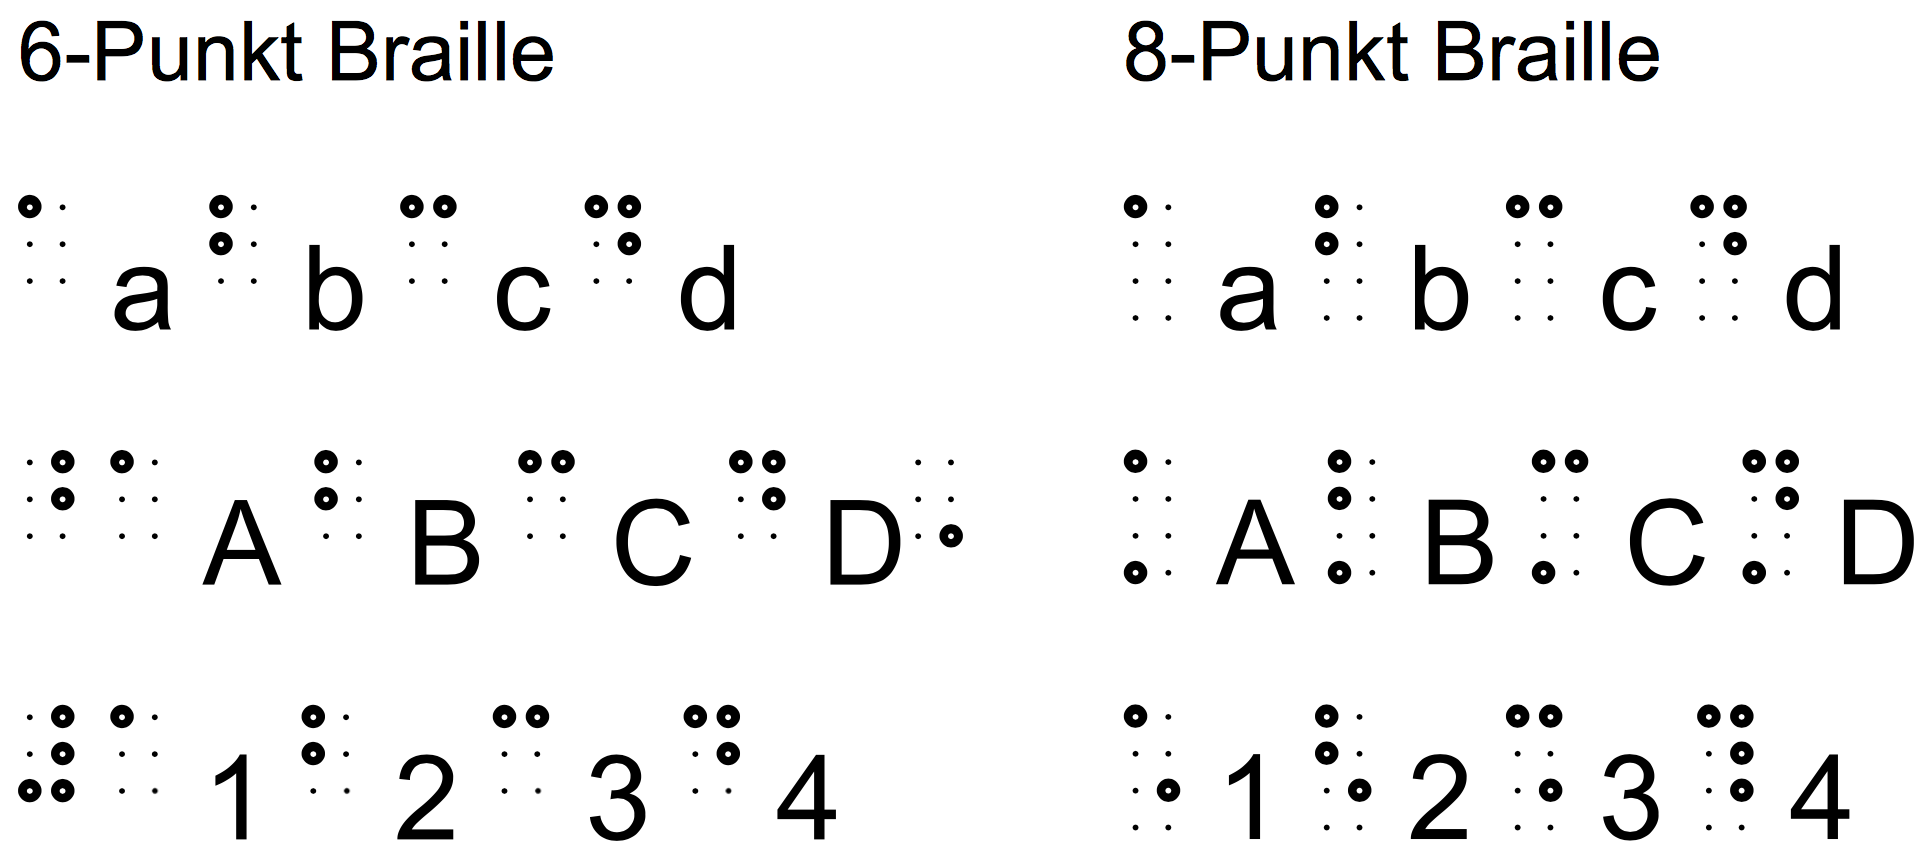
\includegraphics[width=0.6\textwidth]{imgs/braille6v8}
\item Arten
\begin{itemize}
\item Basisschrift: jedes Zeichen 1 Braillebuchstabe
\item Vollschrift: häufige Lautgruppen sind eigene Braillezeichen, 5-10\% Verkürzung gegenüber Basisschrift
\item Kurzschrift: wie Steno, 30-40\% gegenüber Vollschrift\\
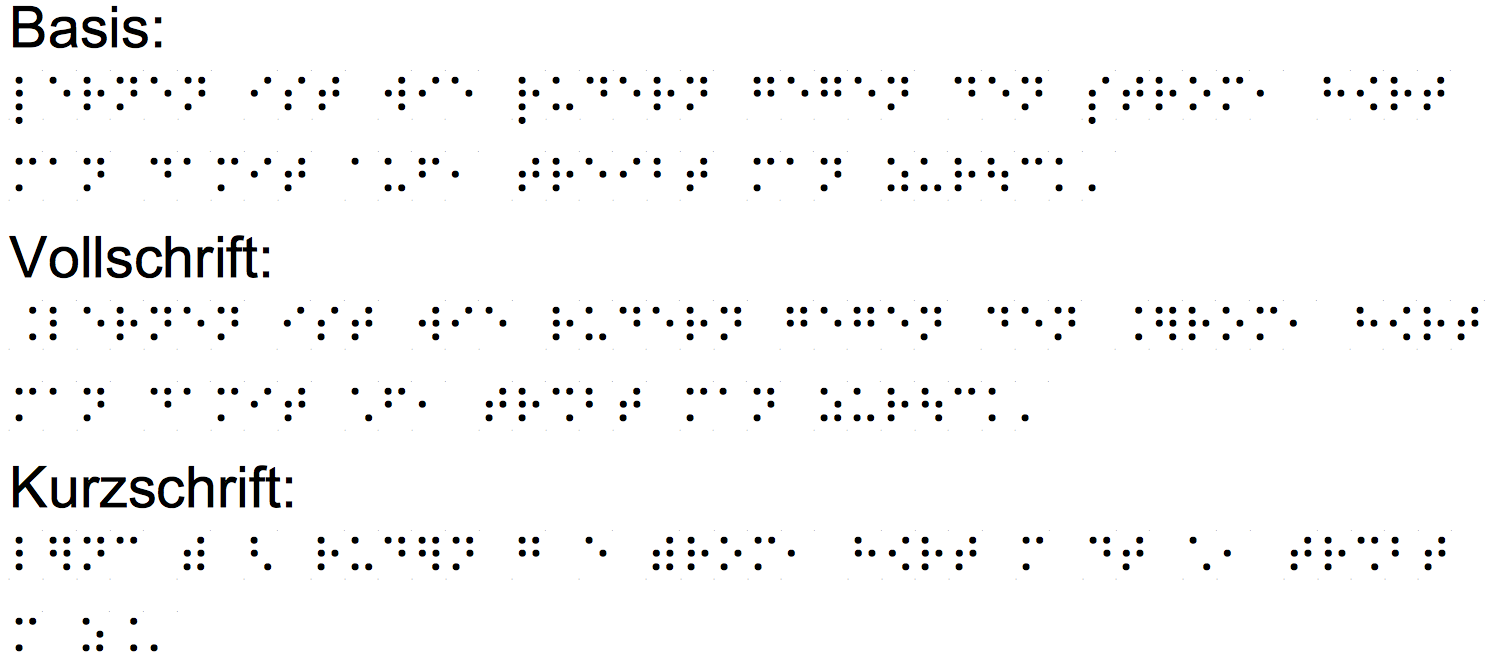
\includegraphics[width=0.6\textwidth]{imgs/braillearten}
\end{itemize}
\item Speziallösungen
\begin{itemize}
\item Marburger Mathematikschrift: klassische 6-Punkt Mathematikschrift, sprachabhängig, sehr kompakte Darstellung, unterstützt mathematisches Verständnis, für Sehende am Bildschirm nicht lesbar
\item LaTeX: weltbekanntes Textsatzsystem mit Beschreibungsmöglichkeit mathematischer Formeln, Einsatz als Mathematikschrift für Blinde aufgrund seiner linearen Darstellung, Problem bei Übersichtlichkeit langer Formeln, beschreibt nicht Mathematik, sondern nur das Layout
\item Lambda (Linear Access to Mathematic for Braille Device and Audio-synthesis): Alternative zu LaTeX, Spezialeditor für Blinde für Mathematik, sehr kompakte Braille Darstellung, Schnittstelle zur graphischen Formeldarstellung, unterstützt mathematisches Verständnis, mathematisches Arbeiten mit Braille-Zeile und Sprachausgabe
\end{itemize}
\item Aktuelle Probleme
\begin{itemize}
\item Gute OCR für Formeln (Formel $\rightarrow$ LaTeX-Code)
\item Sprachsynthese für Formeln
\item Aufbau eines Korpus mit Mathe-Formeln: Sonderzeichen, sequenzielles Lesen, Mangel an Überblick bei Vorlesen von LaTeX-Quellcode $\rightarrow$ Aufbau eines Korpus mit Mathematik-Formeln
\item Musikzugang für Blinde: grafische 2D-Darstellung für Sehende, serielle, 1D-Darstellung für Blinde, Problem vergleichbar mit Mathematikschrift, gleichzeitig spielen und lesen nicht möglich, große Barriere zwischen blinden und sehenden Musikern $\rightarrow$ Beschreibungssprchen für Musiknoten ABC und Lillypont
\end{itemize}
\end{itemize}
\newpage
\section{Assistive Technologien für den Informationszugang}

\subsection{Hilfsmittel für Sehbehinderte}

\begin{itemize}
\item Spezialtastaturen (sehr kontrastreich)
\item Scanner: klassische Scanner für Sehbehinderte, angepasste Scanner mit Braillemarkierung bzw. Sprachausgabe für Blinde
\item FingerReader: MIT entwickelt Lesegerät für Blind mit 3D-Drucker
\item Digitale Lupen\\ 
\begin{minipage}[c]{0.55\textwidth}
\begin{itemize}
\item Zoomfaktor 2x bis 20x
\item Displaygrößen bis 8 Zoll
\item Falschfarbdarstellung
\item Speicherfunktion
\item Neue Modelle auch Texterkennung mit Sprachausgabe
\end{itemize}
\end{minipage}
\begin{minipage}[c]{0.3\textwidth}
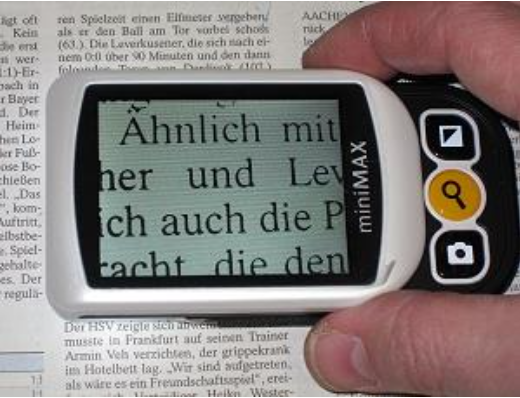
\includegraphics[width=\textwidth]{imgs/lupe}
\end{minipage}
\item Bildschirmlesesysteme\\
\begin{minipage}[c]{0.55\textwidth}
\begin{itemize}
\item Kombinierte Kamera-Bildschirm-Systeme
\item Monitore von 9" bis 47" im Einsatz
\item Zoom 2x bis 100x
\item HD-Auflösung
\item X-Y-Tische (verschiebbare Tische durch Arretierung) zum Teil integriert
\item Neue Modelle auch mit Texterkennung und Sprachausgabe bzw. Sprachsteuerung
\item Falschfarbdarstellung
\item Spiegeldarstellung
\end{itemize}
\end{minipage}
\begin{minipage}[c]{0.3\textwidth}
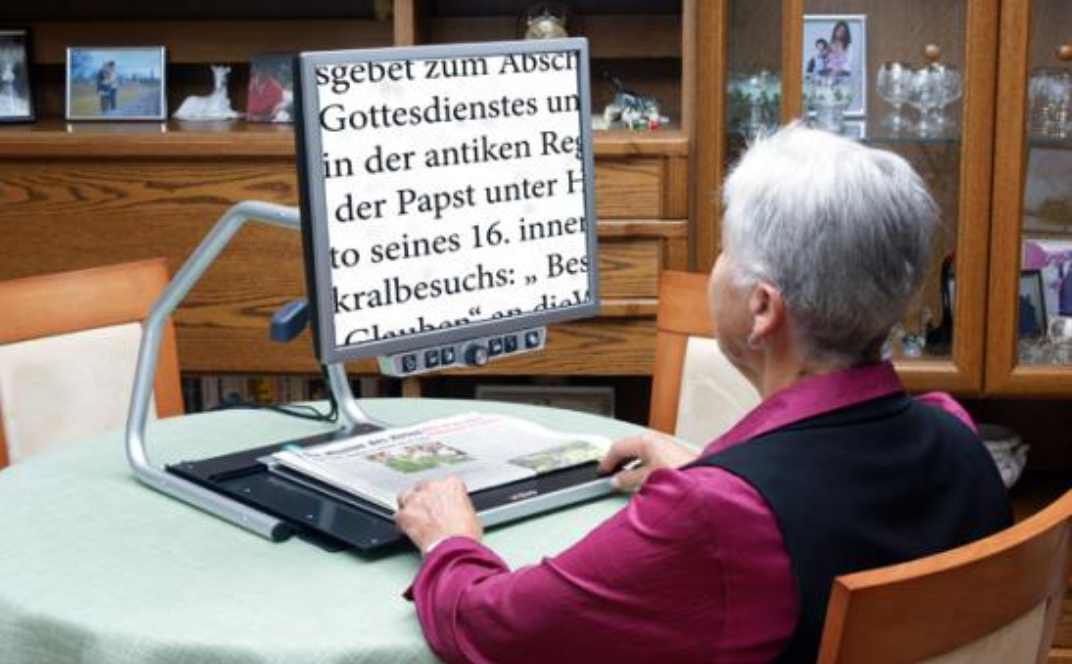
\includegraphics[width=\textwidth]{imgs/bildschirmleser}
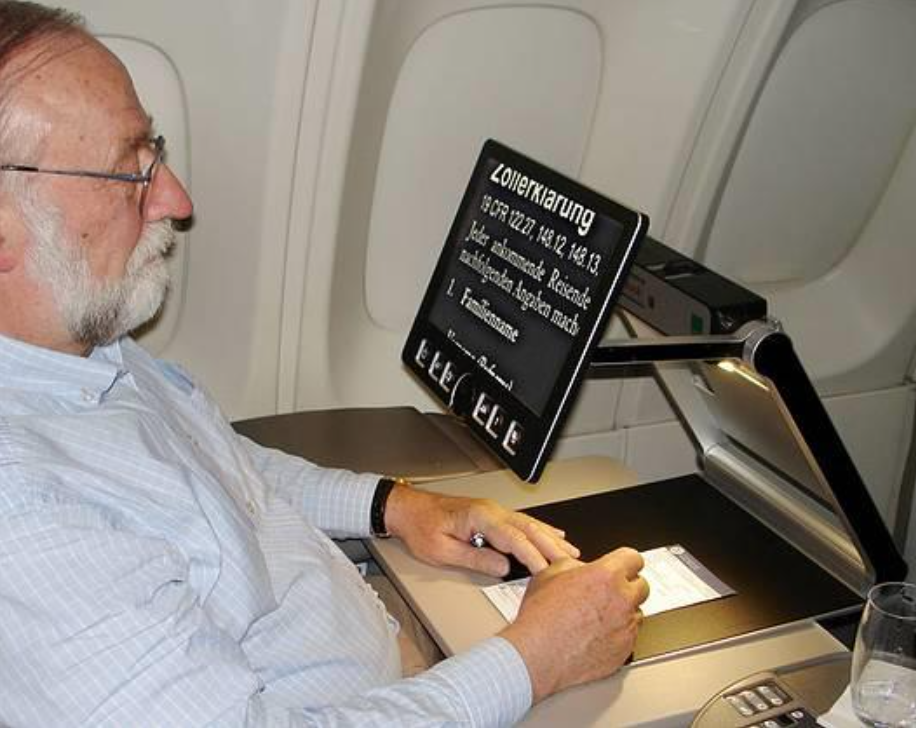
\includegraphics[width=\textwidth]{imgs/bildschirmleser2}
\end{minipage}
\item Kameralösungen\\
\begin{minipage}[c]{0.55\textwidth}
\begin{itemize}
\item Portable Systeme
\item Verwendung mit PC bzw. direkt an einem Monitor
\item Technische Details vergleichbar mit Kameralesesystemen
\item Vorteil: Direkte Archivierung von Dokumenten/Videos am PC
\end{itemize}
\end{minipage}
\begin{minipage}[c]{0.3\textwidth}
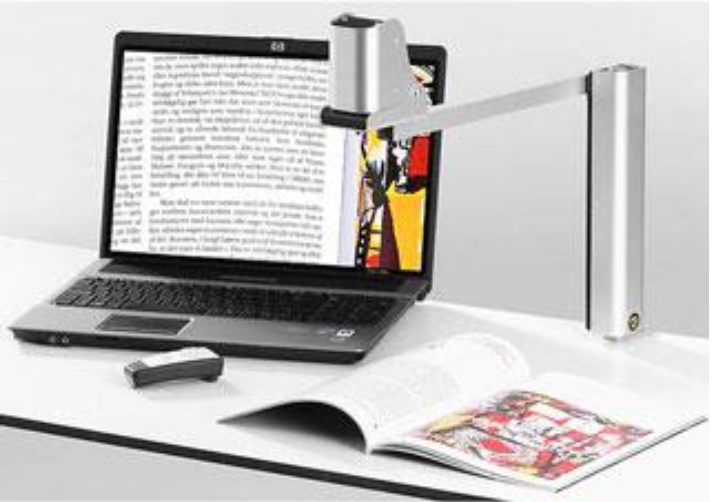
\includegraphics[width=\textwidth]{imgs/kamera}
\end{minipage}
\end{itemize}

\subsection{Hilfsmittel für Blinde}

\begin{itemize}
\item Braillebücher
\item Auditive Materialien (Kassetten, CDs, MP3)
\item DAISY (Digital Accessible Information System)
\begin{itemize}
\item weltweiter Standard für navigierbare, zugängliche Multimedia-Dokumente seit 1992
\item neues digitales Medium, da Audio-CD aus Speicher- und Navigationsgründen für vollständig aufgesprochene Hörbücher ungeeignet
\item bis zu 40 Stunden Ton, Leser kann abhängig von Hierarchiestufen blättern
\item DAISY ist in EBook-Standard EPUB (seit Version 3.0) integriert
\end{itemize}
\item Brailleschreibmaschine
\item Braillezeile: viele Hersteller und Versionen, verschiedene Anzahl an Buchstaben (20, 40, 80), mobile Lösungen (Bluetooth) oder Kabel
\item Screenreader
\item Taktile Grafiken
\item Zeichenbrett
\end{itemize}

\subsection{Drucktechniken für Blinde}

\begin{itemize}
\item Prägen (Drucker 2.000 - 90.000€, Papier wenige Cent)
\item Schwellpapier: spezielle Papierversion zur Erzeugung taktiler Grafiken für Blinde, auf Trägerpapier befindet sich thermoplastische PVC-Schicht, regulär bedrucktes Dokument wird mit UV-Licht beleuchtet, sodass Papier schwillt und ertasten lässt (Drucker unter 100€, Fixierer 1.500€, Papier 2€/Blatt)
\item Tiefziehverfahren: auf gefräste Holzspanplatte wird Kunststoffplatte angepresset und durch Hitze im Gerät zieht sich Kunststoff in das gefräste Objekt (Geräte mehrere 1.000€, Folie wenige Cent, Erstellung großer Aufwand)
\end{itemize}

\subsection{Moderne Ansätze zur Informationsaufnahme}

\begin{itemize}
\item Zweidimensionale taktile Displays
\item Mikrofluides Brailledisplay
\item Carbo-Wachs-Röhrchen
\end{itemize}

\section{IT für den Informationszugang}

\subsection{Softwarelösungen für Sehbehinderte}

\begin{itemize}
\begin{minipage}[c]{0.55\textwidth}
\item Vergrößerungssoftware: flexible Vergrößerung, Font Glättung, Bild-Schärfung, Verfolgung (automatisches Verfolgen des interessanten Bildschirmbereichs), Vergrößerungsfenster, Farbverstärkung, -erweiterung, einstellbarer Mauszeiger und Cursor, Fokus Hervorhebung (z.B. Umrandung), Fokus Echo (z.B. automatisches Vorlesen von gerade aktiven Controls), Maus Echo (z.B. Informationen unter Mauszeiger vorlesen), WebReader (relevante Informationen einer Webseite werden gefiltert), Probleme: fehlende Übersicht da Fullscreen, Abhängigkeiten von Maus und Tastatur
\end{minipage}
\begin{minipage}[c]{0.35\textwidth}
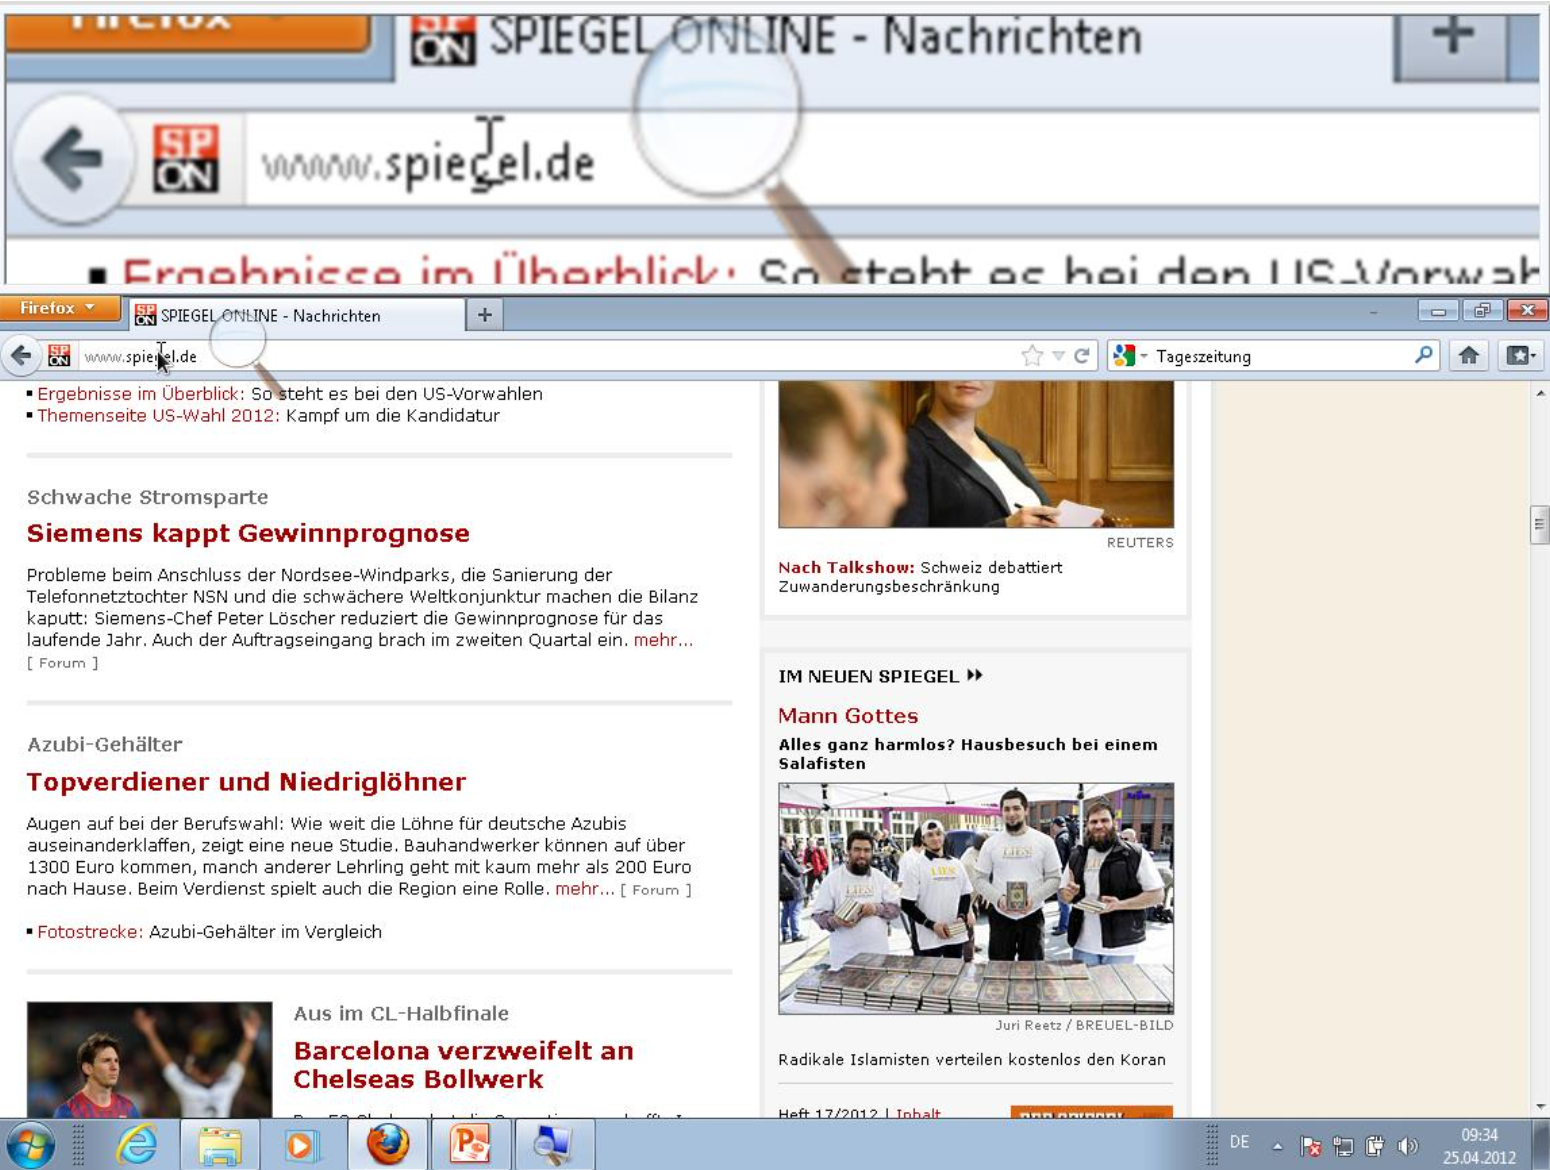
\includegraphics[width=\textwidth]{imgs/softwarelupe}
\end{minipage}\\ 
\begin{minipage}[c]{0.55\textwidth}
\item Eye-Tracking - Probleme: individuelle Anpassung (Farben, Vergrößerung, Dimensionen), Anpassung an Augenerkrankung (Nystagmus: zittern, Schielen, ein blindes Auge), Berücksichtigung der Tagesform, Wechsel zwischen Scan- und Arbeitsmodus
\end{minipage}
\begin{minipage}[c]{0.35\textwidth}
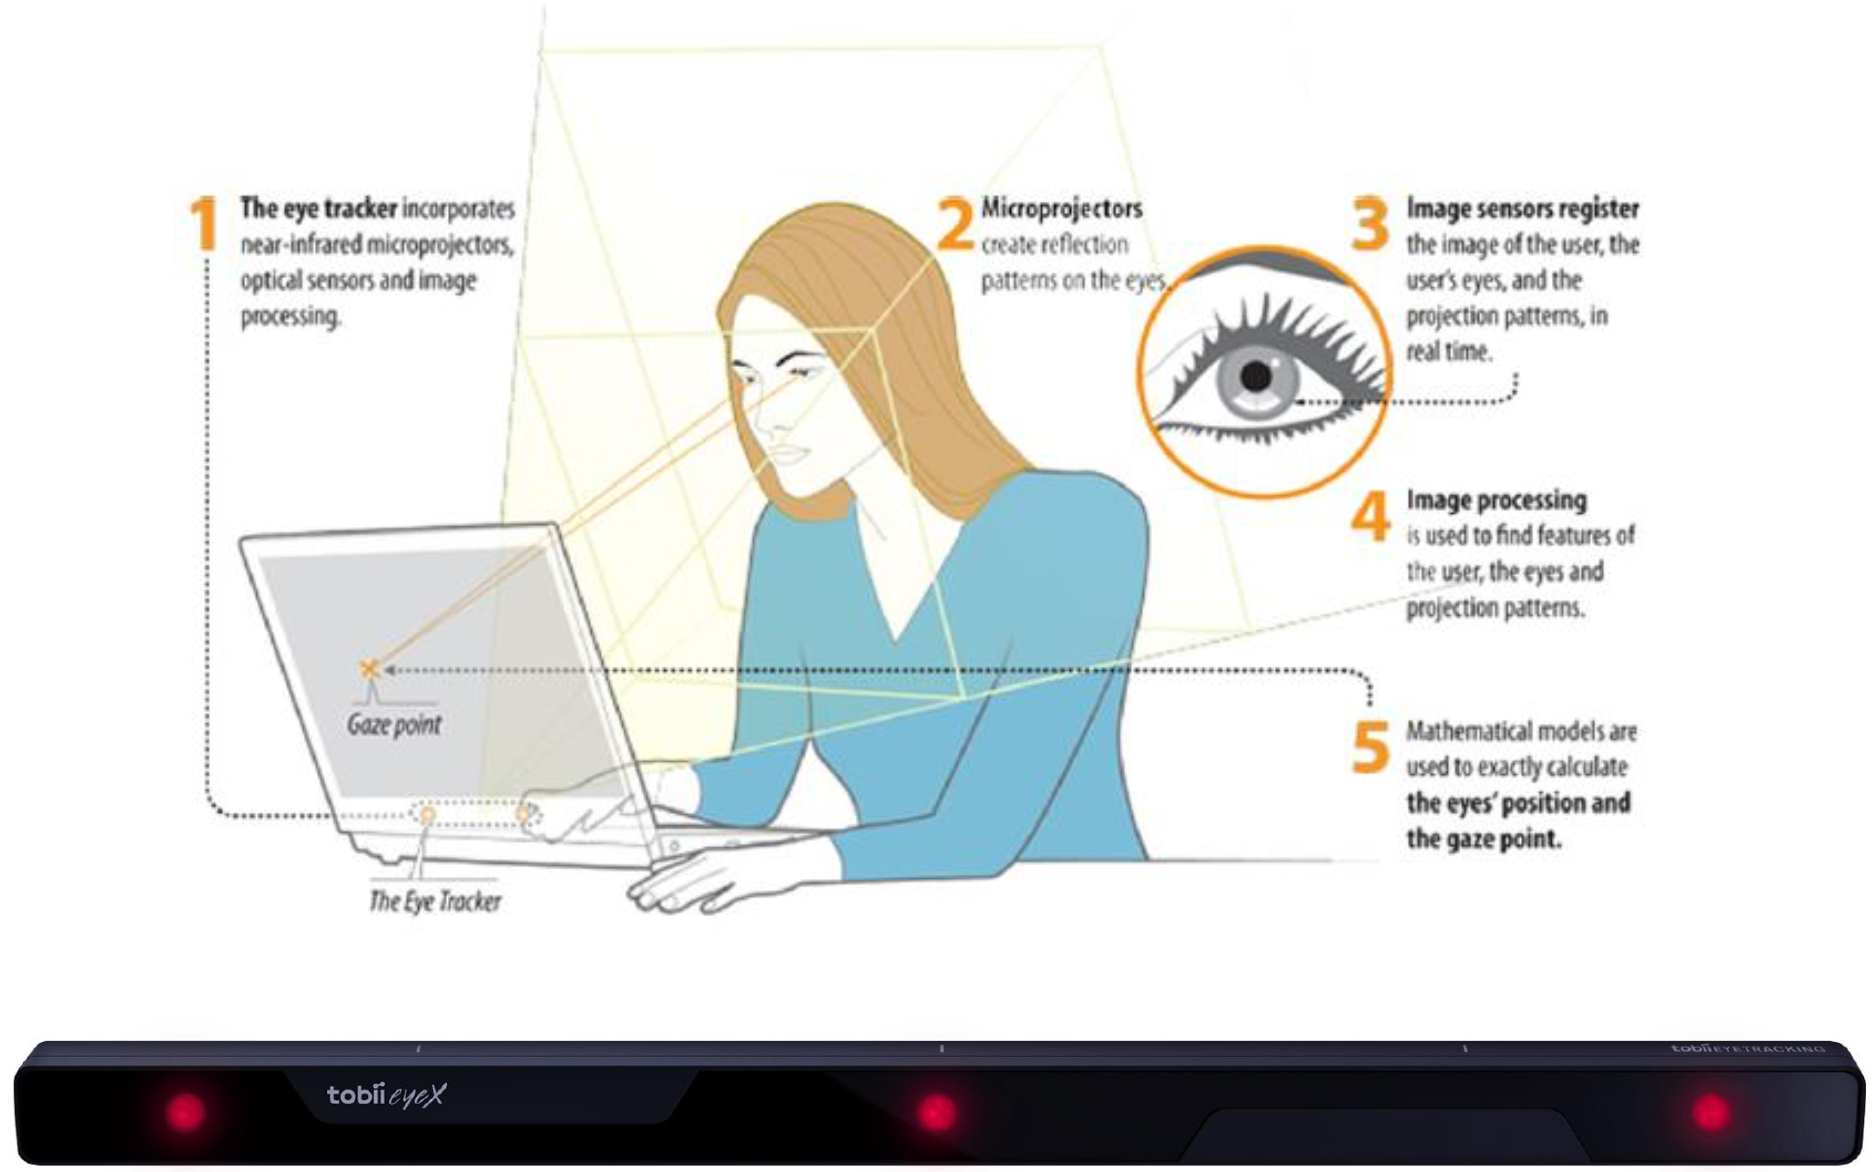
\includegraphics[width=\textwidth]{imgs/eyetracking}
\end{minipage}
\end{itemize}

\subsection{Sprachein-/ausgabe}

\begin{itemize}
\item Text wird in den Rechner bzw. das moble Endgerät eingesprochen und erkannt
\item Beispiele: Dragon NaturallySpeaking, Windows Spracherkennung, Google Now, Siri
\item TextToSpeech(TTS) Software (z.B. Balabolka, TalkBack (Android), VoiceOver (iOS)): Probleme bei Mathematik, Aufbau eines Korpus mit Mathe-Formeln
\end{itemize}

\subsection{Softwarelösungen für Blinde}

\begin{itemize}
\item Screenreader vermittelt Information die gewöhnlich auf dem Bildschirm ausgegeben werden mithilfe nicht-visueller Ausgabegeräte (Soundkarte oder taktil über Braillezeile), Beispiele: NVDA, Jaws, WindowEyes, Orca, VoiceOver
\item Optische Zeichenerkennung (OCR) - Abbyy Finereader, Omnipage
\item InftyReader: OCR für mathematische Ausdrücke und Dokumente (basiert auf Abby Finereader Plugin) - automatische Umwandlung von wissenschaftlichen Dokumenten in Braille
\item ChattyInfty3: Editor für wissenschaftliche (mathematische) Dokumente mit Sprachausgabe
\end{itemize}

\subsection{Aufbereitung von Dokumenten/Informationen/Grafiken}

\begin{itemize}
\item Dokumente
\begin{itemize}
\item PDF/UA-Standard zur barrierearmen Aufbewahrung von Dokumenten (UA: Universal Accessibility) beschreibt erstmalig und einheitlich die Anforderungen an barrierefreie PDF-Dokumente.
\item PAD 2 - PDF Accessibility Checker
\item Warum UA - Alle Menschen sollen selbstständig und gleichberechtigt Informationen in PDF-Dokumenten wahrnehmen und nutzen können (PDF-Dokumente ohne fremde Hilfe nutzen, ein Ziel im Dokument auf einfacheund direkte Weise und in einer angemessenen Zeit erreichen, PDF-Dokumente in gleich hpher Qualität nutzen wie für Menschen ohne Einschränkungen)
\item Vorteile: Screenreader benötigen Strukturinformationen zur Navigation und Alternativtexte für grafische Elemente, Strukturinformation erleichtert auch den Export in andere Formate (ePub, HTML, Word)
\item Hindernisse in PDFs: Text als Bild, Struktur nur visuell erkennbar, falsche Lesereihenfolge, Grafiken ohne Alternativtexte, Dokumentsprache nicht definiert, Überschriften von Tabellen nicht formatiert, Aufzählungen nicht formatiert
\item PDF barrierefrei machen: Tags definieren, Lesereihenfolge definieren
\item PAVE führt Korrektur an PDF-Dateien durch und erzeugt so barrierefreie PDF-Dokumente
\item Tipps für barrierefreie PDFs
\begin{itemize}
\item Tagged PDF (z.B. Überschriften, Absätze, Listen)
\item Logische Lesereihenfolge
\item Umfließen
\item Alternativtext
\item Lesezeichen
\item Sprachauszeichnungen
\item Automatische Prüfung
\end{itemize}
\end{itemize}
\item Grafiken
\begin{itemize}
\item Herausforderungen für Grafikumsetzung und blinde Nutzer: Technische Studienfächer beinhalten große Menge an Grafiken und Bildern, Grafikbeschreibung bedarf detailiertem Wissen im Fachgebiet, Beschreibung soll elektronisch vorliegen, damit sie im jeweiligen Lernmedium auch zukünftig zur Verfügung steht
\item rein textuell über Bildbeschreibung
\item textuell und taktil: Reduktion des grafischen Inhalts (Entfernen von Überschriften, Markierungen, Legenden,..., Entfernen unnötiger und verwirrender Linien, Verbreiterung der Linien)
\item Beschreibung der Grafik über einfache und leicht verständliche Wörter, Art/Typ und Struktur der Grafik, Anordnung der Elemente, auf gelöschte Informationen hinweisen
\end{itemize}
\item Zukunft: ePub 3.x $\rightarrow$ One4All: ein Dokument für alle mit Umschalten für normale, sehbehinderten und blinden Version
\end{itemize}

\section{Richtlinien}

Barrierefreiheit im Web
\begin{itemize}
\item immer mehr Informationen im WWW
\item Fokus von vielen Organisationen liegt dabei häufig auf Design und Reichweite
\item Problem: Zugänglichkeit oft vernachlässigt
\end{itemize}

\subsection{Web Content Accessibility Guidelines (WCAG)}

\begin{itemize}
\item Richtlinie für barrierefreie Webinhalte beschreibt welche Anforderungen ein barrierefreies Web-Angebot erfüllen muss
\item Ausgearbeitet durch Web-Accessibility Initiative (WAI) des World Wide Web Consortiums (W3C)
\end{itemize}

\subsubsection{WCAG 1.0}

\begin{itemize}
\item 1999 veröffentlicht
\item Grundlage für BITV (Deutschland) und auch in vielen anderen Ländern
\item 14 Richtlinien mit 3 Prioritäten
\begin{itemize}
\item Priorität 1: grundlegendste Ebene der Web-Zugänglichkeit
\item Priorität 2: Adressiert die größten Barrieren für Benutzer mit Behinderungen
\item Priorität 3: Signifikante Verbesserungen der Web-Zugänglichkeit
\end{itemize}
\end{itemize}

\subsubsection{WCAG 2.0}

\begin{itemize}
\item basiert auf WCAG 1.0
\item so konzipiert, dass sich weitgehend auf verschiedene Webtechniken der Gegenwart und Zukunft anwenden lassen sowie mit einer Kombination aus automatisierten Tests und der Evaluation durch Menschen testbar sind
\item Richtlinien sind detailierter festgelegt
\item ISO Standard
\item beschreibt 4 Prinzipien mit 12 Richtlinien
\begin{enumerate}[label*=\arabic*.]
\item Wahrnehmbar: Informationen und Komponenten der Benutzerschnittstelle müssen für Benutzer wahrnehmbar sein
\begin{enumerate}[label*=\arabic*.]
\item Textalternativen für alle Nicht-Text-Inhalte, so dass diese in andere vom Benutzer benötigte Formen geändert werden können
\item Zeitbasierte Medien: Alternativen (z.B. Untertitel, Audiodeskription) zur Verfügung stellen
\item Anpassbar: Inhalte sollen auf verschiedene Arten darstellbar sein (z.B. einfacheres Layout), ohne dass Informationen oder Struktur verloren gehen
\item Unterscheidbar: Informationen von Hintergrund trennen
\end{enumerate}
\item Bedienbar: Elemente der Benutzerschnittstelle und Navigation müssen bedienbar sein
\begin{enumerate}[label*=\arabic*.]
\item Per Tastatur zugänglich: alle Funktionalitäten per Tastatur zugänglich
\item Ausreichend Zeit
\item Anfälle: Verhindern der Möglichkeit für Anfälle (z.B. blitzende Bilder)
\item Navigierbar: Hilfsmittel zum navigieren, Inhalte zu finden und zu bestimmen, wo sie sich befinden
\end{enumerate}
\item Verständlich: Informationen und Funktionen der Benutzerschnittstelle müssen verständlich sein
\begin{enumerate}[label*=\arabic*.]
\item Lesbar
\item Vorhersehbar
\item Hilfestellung bei der Eingabe: Hilfe Fehler zu vermeiden und zu korrigieren
\end{enumerate}
\item Robust: Inhalte müssen robust genug sein, sodass diese durch eine Vielzahl von Benutzeragenten verlässlich interpretiert werden können
\begin{enumerate}[label*=\arabic*.]
\item Kompatibel: Kompatibilität mit aktuellen und zukünftigen Benutzeragenten, einschließlich assistierender Techniken
\end{enumerate}
\end{enumerate}
\item jede Richtlinie hat prüfbare Refolgskriterien (A, AA und AAA)
\begin{itemize}
\item A: grundlegendste Merkmale zur barrierefreien Webgestaltung
\item AA: beschäftigt sich mit den größten und häufigsten Barrieren für behinderte Nutzer
\item AAA: höchste und komplexeste Ebene der Web-Zugänglichkeit
\item meist ist AA plus etwas AAA der beste Kompromiss (AA ist Standard für öffentliche Webseiten)
\end{itemize}
\item größtenteils unabhängig von der Webtechnologie
\end{itemize}

\subsection{Barrierefreie-Informationstechnik-Verordnung (BITV)}

\begin{itemize}
\item Barrierefreiheit im Behindrtengleichstelungsgesetz definiert
\item Jedes Bundesland hat eigendes Behindertengleichstellungsgesetz und Regelungen für barrierefreie Informationstechnik
\item BITV: das 2002 in Kraft getretene Behindertengleichstellungsgesetz machte auch eine Rechtsverordnung des Bundes erforderlich, welche im Detail regeln soll, welche Maßnahmen zum Umsetzen des Gleichstellungsgesetzes zum Beispiel für Internetseiten des Bundes notwendig sind.
\item seit 2011: BITV 2.0, orientiert sich an internationalen Standards der WAI des W3C
\item Prinzipien
\begin{enumerate}
\item Wahrnehmbar: Textalternativen, zeitgesteurte Medien, Anpassbarkeit der Darstellung, Unterscheidung Vorder- und Hintergrund
\item Bedienbar: Tastaturbedienbarkeit, ausreichend Zeit, Anfälle vermeiden, Orientierung unterstützen
\item Verständlich: Lesbarkeit, Vorhersehbarkeit, Fehler vermeiden helfen
\item Robust: Kompatibilität
\end{enumerate}
\end{itemize}

\subsection{Unterschiede}

\begin{itemize}
\item WCAG ist nur eine Richtlinie, wobei niemand zur Einhaltung dieser verpflichtet ist
\item Durch BITV wird verpflichtet, dass Oberflächen barrieregerecht gestaltet werden
\end{itemize}

\subsection{Universal Design}

\begin{itemize}
\item Universelles Design und Design für Alle umfassen die Erkenntnisse und Verfahrensweisen, nach denen Produkte, Umgebungen, Dienstleistungen und Informationen für die größtmögliche Zielgruppe gestaltet werden können. Dabei soll der Bedarf an zusätzlichen notwendigen Hilfestellungen aller Art möglichst reduziert werden.
\item Prinzipien des Universellen Designs
\begin{enumerate}
\item Breite Nutzbarkeit: Design soll für Menschen mit unterschiedlichen Fähigkeiten nutzbar und marktfähig sein
\item Flexibilität in der Benutzung: Design soll eine breite Palette individueller Vorlieben und Möglichkeit unterstützen
\item Einfache und intuitive Benutzung: Benutzung des Designs soll leicht verständlich und unabhängig von der Erfahrung, dem Wissen, den Sprachfähigkeiten oder der momentanen Konzentration des Nutzers sein
\item Sensorisch wahrnehmbare Informationen: Design soll dem Benutzer notwendige Informationen effektiv zur Verfügung stellen und zwar unabhängig von der Umgebungssituation oder den sensorischen Fähigkeiten des Benutzers
\item Fehlertoleranz: Design soll Risiken und die negativen Konsequenzen zufälliger oder unbeabsichtigter Aktionen minimieren
\item Niedriger körperlicher Aufwand: Design soll effizient und komfortabel mit einem Minimum von Ermüdung benutzt werden können
\item Größe und Platz für Zugang und Benutzung: eine angemessene Größe sowie Platz für den Zugang, die Erreichbarkeit, die Manipulation und die Benutzung soll vorgesehen werden und zwar unabhängig von der Größe des Benutzers, seiner Haltung oder Beweglichkeit
\end{enumerate}
\end{itemize}

\section{Barrierefreie Webseiten}

\subsection{Grundlagen}

\begin{itemize}
\item HTML vs XHTML: W3C empfiehlt XHTML 1.0, da diese Spezifikation XML-basiert und somit kompatibel mit anderen W3C-Standards ist.
\item XML (eXtensible Markup Language): Auszeichnungssprache zur Darstellung hierarchisch strukturierter Daten in Form von Textdateien
\item CSS macht die Webseite zugänglicher für ein breites Spektrum von Geräten, erleichtert umfangreiche Änderungen, schafft kleinere Dateien und ermöglicht ein bedüfnisorientiertes Anpassen.
\item HTML5 und CSS3 bringen Webseiten mit neuen semantischen Elementen und anspruchsvollen Formatierungseffekten auf den neuesten Stand. Kombiniert können beide Technologien ein barrierefreies, nutzerfreundliches Webdesign unterstützen.
\item SVG (Scalable Vector Graphics): Gestaltung textbasierter, interaktiver und geräteunabhängiger Multimedia genutzt werden
\item SMIL (Synchronized Multimedia Integration Language): kann für die Synchronisation von Video, Untertiteln und Audiodeskriptoren verwendet werden.
\end{itemize}

\subsection{HTML Negativ-/Positiv-Beispiele}

\begin{center}
    \begin{tabular}{| p{4.5cm} | p{5cm} | p{5cm} |}
    \hline
    Beispiel & gute Umsetzung & schlechte Umsetzung \\ \hline
    Überschriften & <h2>Überschrift 2</h2> & <strong>Überschrift 2</strong> \\ \hline
    Listen und Aufzählungen & <ul><li>...</li></ul> & Auflistung mit einfachem Zeilenumbruch und Bindestrich \\ \hline
    Tabellen & Inhaltsübersicht und Kopfzeilen markieren & Tabelle als Textrahmen oder als Positionswerkzeug \\ \hline
    Transparente Bilder als Positionswerkzeug & Abstände über CSS & transparente Bilder als Positionswerkzeug \\ \hline
    Links & externe Links kenntlich gemacht & keinerlei Aussagekraft wo ein Link hinführt \\ \hline
    Abbildungen und Grafiken & ALT/TITLE/LONGDESC & keine Beschreibung \\ \hline
    \end{tabular}
\end{center}

\subsection{Accessibility-API/-Tree/ARIA}

\begin{itemize}
\item Barrierefreihehit einer Anwendung ist davon abhängig, wie sie über eine Accessibility-API den Accessibility-Tree mit Informationen befüllt
\item APIs: Microsoft Active Accessibility (MSAA) auf Windows, Linux Accessibility Toolkit und Assistive Technology - Service Provider Interface auf Linux, Mac OS X Accessibility Protocol auf macOS und iOS, Java Accessiblity API (JAAPI)
\item Accessiblity-Tree: Schnittstelle des Betriebssystems
\item Document Object Model (DOM)
\item Off screen model: heuristisches Verfahren in dem Screenreader die Kommunikation zwischen Browser und Betribssystem auswerten
\item ARIA (Accessible Rich Internet Application) - Webstandard des W3C
\begin{itemize}
\item mit ARIA-Atrributen können u.a. Komponenten, die in HTML und anderen Auszeichnungssprachen nicht spezifiert sind, so angereichert werden, dass der Browser damit den Accessibility-Tree sinnvoll befüllen kann
\item werden mittlerweile von Browser und Betriebssysteme ausreichend unterstützt
\item sind leicht zu verstehen
\item schließen die Lücke zwischen HTML und JavaScript einerseits und zwischen HTML und dem Betriebssystem andererseits
\item beeinflussen weder die visuelle Darstellung noch das Verhalten im Browser
\item Rollen und Attribute
\begin{itemize}
\item landmark roles um Regionen einer Webseite zu bestimmen
\item document structure roles um fehlende Semantik einem Element hinzuzufügen
\item widget roles um komplexere Komponenten, die größtenteils in HTML5 nicht abgebildet werden können, semantisch zu identifizieren
\end{itemize}
\end{itemize}
\end{itemize}

\subsection{Validierungshilfen und weitere Tools}

\begin{itemize}
\item Active Accessibility Object Inspector
\item Aviewer
\item Accessibility Inspector (macOS)
\item AccProbe (Linux)
\end{itemize}

\section{Barrierefreie Softwareentwicklung}

Barrierefreie Software ist eine Software die für alle Menschen unabhängig irgendwelcher Einschränkungen bedienbar ist.

\subsection{Grundlagen und Richtlinien}

\begin{itemize}
\item Eine barrierefreie Software sollte für Menschen mit Körperbehinderung und bedingt auch für Menschen mit geistigen Behinderungen und Lernbehinderungen bedienbar sein.
\item Außerdem sollte eine barrierefreie Software auch von Menschen im fortgeschrittenen Alter bedienbar sein.
\item Eine barrierefreie Software sollte von allen Menschen bedient werden können!
\item Eine barrierefreie Software macht es allen Computernutzern einfach die Software zu bedienen!
\item \textbf{Auch die UN-Konvention nennen und betonen, dass der ungehinderte Zugang zu Informationen und Kommunikation ein Menschenrecht ist!}
\item Beispiele für Barrieren
\begin{itemize}
\item Blind, Sehbehindert (bisher behandelt, aber...)
\item Taub/Hörbehinderung
\begin{itemize}
\item Untertitel (manuell/automatisch erstellt)
\item Kommunikation $\rightarrow$ SMS, Emmail, WhatsApp, Chat
\item Text-Transkription (z.B. in Vorlesungen)
\item Wecker? Rauchmelderalarm? Türklingel? Telefon? z.b. Bett-Vibrator unter dem Kopfkissen, Blitzlichtlampen für Alarmsignalisierung
\item Lautsprecherdurchsagen in Straßenbahnen
\item Intelligente Hörgeräte (Geräuschfilterung, ggf. Speech-To-Text)
\end{itemize}
\item Mobilitätseinschränkung und Geschicklichkeitsprobleme
\item Sprachbeeinträchtigung
\item Dyslexie
\begin{itemize}
\item beeinflusst Fähigkeit zu lesen, zu buchstabieren und Zahlen zu verwenden
\item Technologie finden, um Passwortschutz und Support zu unterstützen
\item Intelligente Fehlerprüfung
\item Technologien finden, die in verschiedenen Einstellungen für verschiedene Aufgaben funktionieren
\item Kreativität im Umgang mit Technologien
\end{itemize}
\item Alter
\end{itemize}
\item Wie kann Barrierefreiheit bei der Programmierung von Software berücksichtigt werden?
\item Wie kann Software hinsichtlich Barrierefreiheit überprüft werden?
\item Gibt es Kriterien für die Beschaffung von barrierefreier Software?
\item Gibt es Richtlinien?
\begin{itemize}
\item Ja, es gibt leider verschiedene Richtlinien: ISO 9241 Ergonomie der Mensch-System-Interaktion – Teil 171: Leitlinien für die Zugänglichkeit von Software (ISO 9241-171:2008)
\item Richtlinien zur barrierefreier Software-Entwicklung mit .net bzw. C\#
\begin{enumerate}
\item Unterstützung der Systemsteurungseinstellungen für Größe, Farbe, Schriftart und Eingabe
\item Unterstützung des Kontrastmodus
\item Bereitstellen eines dokumentierten Tastaturzugriffs auf alle Features
\item Visuelle und programmgesteuerte Anzeige der Position des Tastaturfokus
\item Vermeidung der Übermittlung wichtiger Informationen allein per Audioausgabe
\end{enumerate}
\item Richtlinien zur barrierefreien Software-Entwicklung für Java von IBM
\begin{enumerate}[label*=\arabic*.]
\item Tastaturbedienbarkeit
\begin{enumerate}[label*=\arabic*.]
\item Alle Softwarefunktionen müssen auch ohne Maus, also nur per Tastatur ausführbar sein
\item Es darf keine Konflikte geben zwischen Ihrer Software und Tastatureingabehilfen des Betriebssystems
\end{enumerate}
\item Informationen über Objekte
\begin{enumerate}[label*=\arabic*.]
\item Bieten Sie eine optische Fokusanzeige an, die den Änderungen des Eingabefokus zwischen den interaktiven Objekten folgt. Diese Fokusanzeige muss programmtechnisch für die assistive Technik zugänglich sein.
\item Liefern Sie semantische Informationen über Objekte der Benutzerschnittstelle. Wenn ein Programmelement aus einem Bild besteht, dann muss die Information, die durch das Bild transportiert wird, auch als Text verfügbar sein.
\item Beschriften Sie Bedienelemente, Objekte, Icons und Bilder. Wenn ein Bild zur Kennzeichnung von Programmelementen benutzt wird, muss die Bedeutung des Bildes in der gesamten Applikation einheitlich sein.
\item Wenn elektronische Formulare in der Software benutzt werden, sollten die Formulare den Menschen, die assistive Technik benutzen, erlauben, auf die Informationen, Feldelemente und Funktionen zuzugreifen, die zum Ausfüllen und zur Abgabe des Formulars, einschließlich aller Anweisungen und Hinweise, notwending sind.
\end{enumerate}
\item Sound und Multimedia
\begin{enumerate}[label*=\arabic*.]
\item Bieten Sie eine Option, um Audio-Warnmeldungen visuell anzuzeigen.
\item Bieten Sie zugängliche Alternativen für wichtige Audio- und Videosequenzen.
\item Bieten Sie eine Option zum Einstellen der Lautstärke.
\end{enumerate}
\item Anzeige
\begin{enumerate}[label*=\arabic*.]
\item Erzeugen Sie Text durch normale Systemfunktionsaufrufe oder eine API (Schnittstelle für Anwendungsprogrammierung), die die Interaktion mit assistiver Technik unterstützen.
\item Benutzen Sie Farbe als eine Ergänzung und nicht ausschließlich, um Informationen zu übermitteln oder Aktionen anzuzeigen.
\item Unterstützen Sie Einstellungen für starken Kontrast für alle Bedienelemente des Benutzerinterfaces und Client-Bereiches.
\item Wenn kundenspezifische Farbanpassung durch das Programm unterstützt wird, bieten Sie vielfältige Farbeinstellungsmöglichkeiten, damit mehrere Kontrastniveaus erzeugt werden können.
\item \textbf{Übernehmen Sie die Systemeinstellungen für Schriftart, Größe und Farbe für alle Steuerelemente der Benutzerschnittstelle.}
\item Bieten Sie eine Option an, die Animationen in einer nicht animierten Form darstellt.
\end{enumerate}
\item Timing
\begin{enumerate}[label*=\arabic*.]
\item Bieten Sie die Möglichkeit, die \textbf{Reaktionszeit auf zeitlich begrenzte Hinweise einzustellen} oder ermöglichen Sie den Verbleib des Hinweises.
\item Verwenden Sie keine leuchtende oder blinkende Texte, Objekte oder andere Elemente mit einem Blitz oder einer Blinkfrequenz größer als 2 Hz und kleiner als 55 Hz.
\end{enumerate}
\end{enumerate}
\item Richtlinien barrierefreie Software-Entwicklung für Java von Oracle
\end{itemize}
\item Allgemeine wichtige Hinweise
\begin{itemize}
\item Tabulatorreihenfolge: Um die Bedienbarkeit der Software auch über Tastatur zu gewährleisten, ist es wichtig auf die Tabulatorreihenfolge zu achten.
\item Shortcuts: Eine weitere Möglichkeit die Bedienbarkeit von Software über Tastatur zu verbessern, ist das vergeben von Shortcuts für Labels, Buttons, Groupboxen und Menüs. Das erstellen eines Shortcuts macht man, in dem man vor einem bestimmten Buchstaben in einer Beschriftung ein \&-Zeichen setzt.
\item Achtung bei individuellen Shortcuts: Keine WCAG Richtlinie aber häufig werden Shortcuts definiert, welche schon anderweitig im System vergeben sind.
\end{itemize}
\end{itemize}

\subsection{Checker für Barrierefreiheit}

\begin{itemize}
\item Wie kann Software hinsichtlich der Barrierefreiheit überprüft werden?
\item Automatisierte Überprüfung ist noch immer schwierig
\item Microsoft und Oracle stellen Tool zur Verfügung um Software auf Barrierefreiheit zu testen
\item Sofrware sollte von Hand überprüfen, um Barrierefreiheit wirklich sicherzustellen (Überprüfen der Software anhand der verwendeten Richtlinien)
\item Als Checkliste hierfür dient die im Anhang C der ``DIN EN ISO 9241-171 Leitlinien für die Zugänglichkeit von Software'' bereitgestellte ``Checkliste zur Beurteilung von Anwendbarkeit und Einhaltung der Anforderungen und Empfehlungen (Konformität)''.
\end{itemize}

\subsection{Beispiele für Programmiersprachen/Oberflächenentwicklung}

Welche Programmiersprachen unterstützen barrierefreie Software-Entwicklung?
\begin{itemize}
\item Java war die erste welche barrierefreie Software-Entwicklung unterstützte.
\begin{itemize}
\item Swing-Komponenten bieten Eigenschaften AccessibleName und AccessibleDescription
\item Diese Texte werden dann vom Screenreader vorgelesen
\item \textbf{JAAPI} ermöglicht eine Art Vereinbarung zwischen einer Java-Anwendung und der Unterstützungstechnologie (wie Screenreader-Software oder Braille-Anzeigegerät)
\item Java Accessibity-Dienstprogramme: Damit können Informationen aus einer Anwendung erfasst und für die Anzeige mit Spezialgeräten weiterverarbeitet werden. Mit ihnen können Untersützungstechnologien komponentenspezifische Ereignisse überwachen und zusätzliche Informationen über das GUI erhalten, zum Beispiel die momentane Mausposition oder, welches Fenster gerade aktiv ist.
\item Java Access Bridge (JAB): Das wichtigste Element, um unter Windows Barrierefreiheit in der Java-Plattform zu ermöglichen. Es wurde in J2SE 1.3 eingeführt.
\item Java Foundation Classes (JFC): Dies ist eine Bibliothek von GUI-Komponenten, in welche JAAPI vollständig implementiert ist.
\end{itemize}
\item Das Microsoft .net-Framework insbesondere C\# unterstützt ebenso die barrierefreie Software-Entwicklung!
\begin{itemize}
\item AccessibleName: Kurzbeschreibung der entsprechenden Komponente
\item AccessibleDescription: Textbeschreibung der visuellen Darstellung dieser Komponente
\item AccessibleRole beschreibt die Aufgabe, die an Eingabehilfen übermittelt wird, zulässige Were in Enum AccessibleRole definiert.
\item AccessibilityObject enthält eine Instanz, die für die Eingabehilfe Informationen über das Steuerelement enthält. Die Eingeschaft ist schreibgeschützt und wird vom Designer festgelegt.
\item AccessibleDefaultActionDescription enthält eine Beschreibung der Standardaktion des Steuerelements. Diese Eigenschaft kann nicht zur Entwurfszeit festgelegt werden, sondern nur per Programmcode.
\item Kontrastmodus: Kontrastmodus des Systems kann in Software übernommen werden
\item Neues Feature: UI Analyse in Visual Studio hilft während der Programmierung typische Fehler in Sachen Barrierefreiheit zu finden und hilft diese zu beheben.
\item Narrator/Windows 10 Sprachausgabe: Windows 10 Screenreader
\end{itemize}
\item Qt
\begin{itemize}
\item QT accessability checklist: Usability, Fonts, Colors, Scalable UI, Sounds, Spelling, Assistive Technology
\item Barrierefreie QT-Anwendungen: Um mit assistiven Technologien zu kommunizieren, muss die QT-GUI für diese verständlich erstellt werden. QT-Anwendungen verwenden das \textbf{QAccessibleInterface}, um Informationen über die einzelnen Elemente der Benutzeroberfläche bereit zu stellen. Im Moment bietet QT Unterstützung für seine Widgets und Widget-Teile, z.B. Schieberegler Griffe, aber die Schnittstelle konnte auch für jede QObject umgesetzt werden. Die Beschreibungen basieren hauptsächlich auf MSAA und sind unabhängig von QT.
\end{itemize}
\item Android
\begin{itemize}
\item Accessibility Features: Android bietet Eingabehilfen und Dienstleistungen die bei der Navigation helfen, einschließlich Sprachausgabe, haptische Rückmeldung oder Gestensteuerung. Android-Entwickler können durch diese Funktionen in ihren Anwendungen profitieren. Android-Entwickler können auch ihre eigenen Anwendungen dadurch zugänglich machen und Funktionen wie Audio-Aufforderung, physikalisches Feedback (Vibration) und alternative Navigationsmodi nutzen.
\item Accessibility Requirements: Gewisse Punkte müssen hierfür erfüllt werden, um die minimalen Anforderungen für eine barrierefreie Anwendung zu gewährleisten (Alternativtexte für GUI-Komponenten, die keinen sichtbaren Text enthalten, Sicherstellen, dass Nutzer mit Hard- oder Softwarebasierenden Lösungen navigieren können, Bei selbstentwickelten Steuerelementen für Nutzerschnittstellen sollen Accessibility Schnittstellen und Inhaltsbeschreiber integriert werden, Audioausgaben müssen immer eine zweite Rückmeldung haben, um hörbehinderte Personen zu unterstützen)
\item Accessibility Recommendations: Empfehlungen um die Zugänglichkeit der Programme sicherzustellen (Android Design Accessibility Guidelines, framework-provided controls benutzen, temporary or self-hiding controls and notifications verhindern)
\end{itemize}
\item iOS
\begin{itemize}
\item Eingabehilfen, Accessibility-APIs, Vielzahl von Entwicklertools und Dienstprogrammen (z.B. VoiceOver)
\item Test auf Accessibility: Test auf realem Gerät oder im iOS Simulator, Accessibility Inspector hilft beim Debuggen der Zugänglichkeiten (läuft innerhalb iOS-Simulator)
\end{itemize}
\item In vielen weiteren liegt es im Ermessen des Entwicklers bzw. am Einsatz von passenden Plugins.
\item Bei den Programmiersprachen C++ und Delphi fehlt eine Unterstützung von Haus aus.
\end{itemize}

\section{Feedbacksysteme und Evaluierung}

Welche Möglichkeiten gibt es, Informationen an sehbehinderte Nutzer zu bringen?
\begin{itemize}
\item Visuell - nur für Sehbehinderte und problematisch alle Seheinschränkungen abzudecken
\item Sprachausgabe - problematisch, Sprachausgabe lenkt von den restlichen Umweltgeräusche bzw. im Gespräch zu sehr ab
\item Möglichkeiten: Sonifikation (Töne) oder Haptik/Vibration
\end{itemize}

\subsection{Akustische Feedbacksysteme}

\begin{itemize}
\item Sonifikation: Verklanglichung ist die Darstellung von Daten in Klängen $\rightarrow$ Klang als Informationskanal (Beispiele: Stethoskop, Geigerzähler)
\item Sonifizierungstechniken
\begin{itemize}
\item Audifikation: direkte Übersetzung von Daten auf ein akustisches Signal, Daten müssen in Signalform sein, EEG (Elektroenzephalographie) zur Vorhersage epileptischer Anfälle, Seismogramm
\item Earcons: überlicherweise melodisches Konstrukt aus einen bis drei Tönen, jedem Earcon wird eine Bedeutung zugewiesen, Assoziationen müssen erst gelernt werden, viele verschiedene Klangparameter veränderbar, angenehmer Klang (Windows-Fehlermeldung, Windows herunterfahren)
\item Auditory Icons: Geräusche ähnlich zu akustischen Ereignissen im Alltag, intuitiv, oft bei Human-Computer Interaktion eingesetzt, Rückmeldung für Eingaben, schwer immer passende Töne zu finden
\item Parameter Mapping Sonification: Abbildung einzelner Datenattribute auf einzelne Klangattribute, Datenverarbeitung, Datentendenz erkennen, Sound Graphs
\item Modellbasierte Sonifikation: aktive (z.B. der Vortrag) und passive Klänge (z.B. Schlag auf den Tisch), künstliche Interaktion mit abstrakten Modellen liefert Geäusche (z.B. oft gedrücktet Button klingt weniger frisch)
\item Spearcons: Text-to-Speech (TTS), 40-50\% schneller abgespeilt, einfach zu produzieren, können theoretisch jeden Vorgang beschreiben, gewöhnungsbedüfrtig, schneller erlernbar, bildhaft
\end{itemize}
\item Anwendungsbeispiele
\begin{itemize}
\item Hinderniserkennung: Langstock (haptisch aber auch auditiv), Bat K Sonar-Cane (Tonhöhe des Echo analog zur Entfernung, direktional, durch Kopfhörer werden Umweltgeräusche verdeckt)
\item Audible High Resolution Ultrasonic Sonar (AHRUS): hörbares Ultraschall Sonar, dessen Echos mit dem menschlichen Ohr wahrgenommen werden können
\item Auditory Graphs: kartesische Graphen, y-Wert auf Tonhöhe abbilden, gibt einen ersten Eindruck über die Funktion, mehr Information durch Interaktion, y = x + sin(x)
\item Soundbeam: ähnlich wie ein Musikinstrument, übersetzt sensorisch erfasste Handbwegungen in Musik und Klang, 2 Ultraschallsensoren
\end{itemize}
\end{itemize}

\subsection{Haptische Feedbacksysteme}

\begin{itemize}
\item Haptische Wahrnehmung
\begin{itemize}
\item Haptische Sensitivität (Bestandteil der Oberflächensensibilität, Wahrnehmung mechanischer Reize in Forum von Druck, Vibration und Gewebsdehnung)
\item Propriozeption (Tiefensensibilität, Fähigkeit die Stellung der Gliedmaßen und die Lage des eigenen Körpers im Raum wahrzunehmen)
\item Kinästhesie (Tiefensensibilität, Fähigkeit Körperbewegungen wahrzunehmen und zu steuern)
\item Viszerozeption (Wahrnehmung der Informationen über Organtätigkeiten)
\item Schmerzwahrnehung (Nozizeption)
\item Tempraturwahrnehmung (Thermorezeption)
\end{itemize}
\item Taktile Wahrnehmung: 
\begin{itemize}
\item Passive Wahrnehmung mechanischer Eindrücke
\item Teil des Tastsinns
\item Oberflächensensibilität: Wahrnehmung von Reizen über in der Haut liegende Rezeptoren, die in Mechano-, Thermo- und Schmerzrezeptoren unterteilt, mit deren Hilfe Druck, Berührung und Vibration sowie Temperatur und Schmerz wahrgenommen werden können
\end{itemize}
\item Taktiles Feedback
\begin{itemize}
\item Vibrotaktile Stimulation: Mit Hilfe von Vibrationen kann man verschiedenste Empfindungen simulieren, zum Beispiel Bewegungen oder auch Oberflächenstrukturen
\item Pneumatische Stimulation: Auch über bestimmte Druckveränderungen auf die Finger oder andere Hautstellen können Reize ausgelöst werden (z.B. Braillezeile)
\item Elektrotaktile Stimulation: Diese Reizentwicklung wird durch kleine Elektroden erreicht. Diese werden auf die Haut angebracht und geben kleine Stromstöße ab
\item Temperaturinformationen: Auch durch verschiedene Temperaturinformationen kann ein taktiles Feedback erreicht werden, zum Beispiel die Übermittlung von Temperaturdifferenzen
\item Nervenstimulation (Functional neuromuscular stimulation FMS): Es ist auch möglich, direkt die Nerven des Benutzers derart anzusteuern, dass eine haptische Wahrnehmung entsteht.
\end{itemize}
\item Force Feedback
\begin{itemize}
\item Fingerbasierende Interfaces: Diese Geräte werden durch Fingerbewegungen gesteuert. Bei dieser Gruppe von Geräten wird meist ein Mauszeiger im Dreidimensionalen gesteuert, mit dem man Objekte anstoßen kann.
\item Handbasierende Interfaces: Bei diesen Geräten wird die Bewegung der Hand ausgewertet. Aber auch Joysticks zählen zu dieser Gruppe.
\item Exoskeletale Interfaces: Die Steuerung erfolgt hier durch Teile des Skeletts. Das Gerät wird so befestigt, dass es die natürlichen Bewegungen des Benutzers registrieren und aufzeichnen kann.
\end{itemize}
\item Beispiele
\begin{itemize}
\item Joysticks oder Lenkräder\\ 
\begin{minipage}[c]{0.55\textwidth}
\item PHANTOM: gehört zu der Gruppe der fingerbasierenden Interfaces. Es wurde am MIT in Boston entwickelt und wird zur Zeit von der Firma SensAble Technologies produziert und vertrieben.
\end{minipage}\qquad
\begin{minipage}[c]{0.35\textwidth}
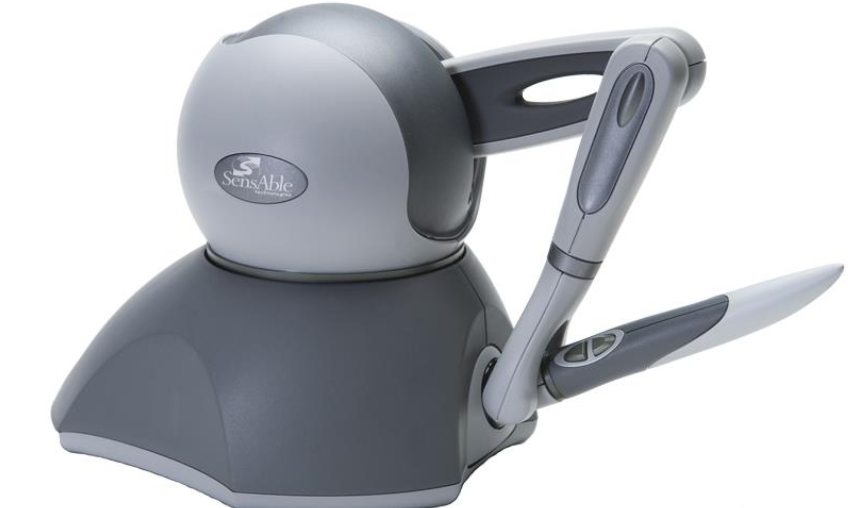
\includegraphics[width=\textwidth]{imgs/phantom}
\end{minipage}
\begin{minipage}[c]{0.65\textwidth}
\item CyberGlove: Sensoren liefern Daten über die Stellung und Ausrichtung der Finger und Gelenke. Die dadurch erhaltenen Informationen werden zu einer graphischen Hand umgerechnet, die sich im virtuellen Raum bewegt und die Bewegungen der realen Hand repräsentiert. Dadurch kann der Benutzer im virtuellen Raum handel und Aktionen durchführen.
\end{minipage}\qquad
\begin{minipage}[c]{0.2\textwidth}
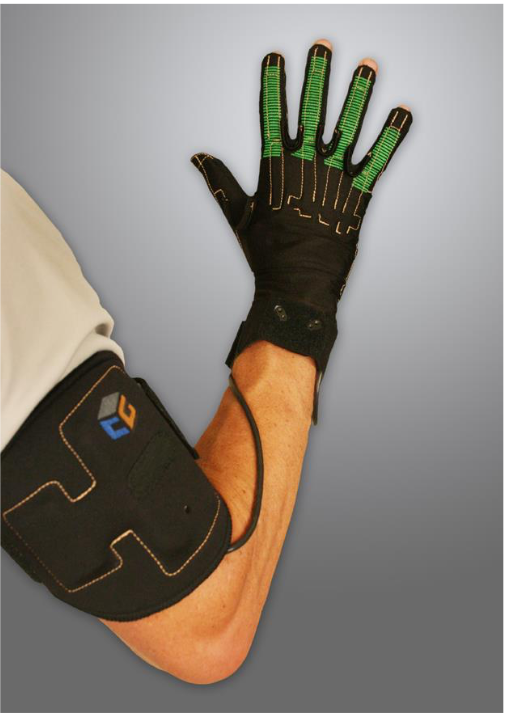
\includegraphics[width=\textwidth]{imgs/cyberglove}
\end{minipage}\\ 
\begin{minipage}[c]{0.65\textwidth}
\item CyberTouch: Erweiterung des CyberGlove. Er vermittelt dem Benutzer ein taktiles Feedback. Um das zu erreichen, ist er mit sechs vibrotaktilen Stimulatoren ausgestattet. Fünf dieser Sensoren sind an den Fingern angebracht, einer auf der Handfläche.
\end{minipage}\qquad
\begin{minipage}[c]{0.2\textwidth}
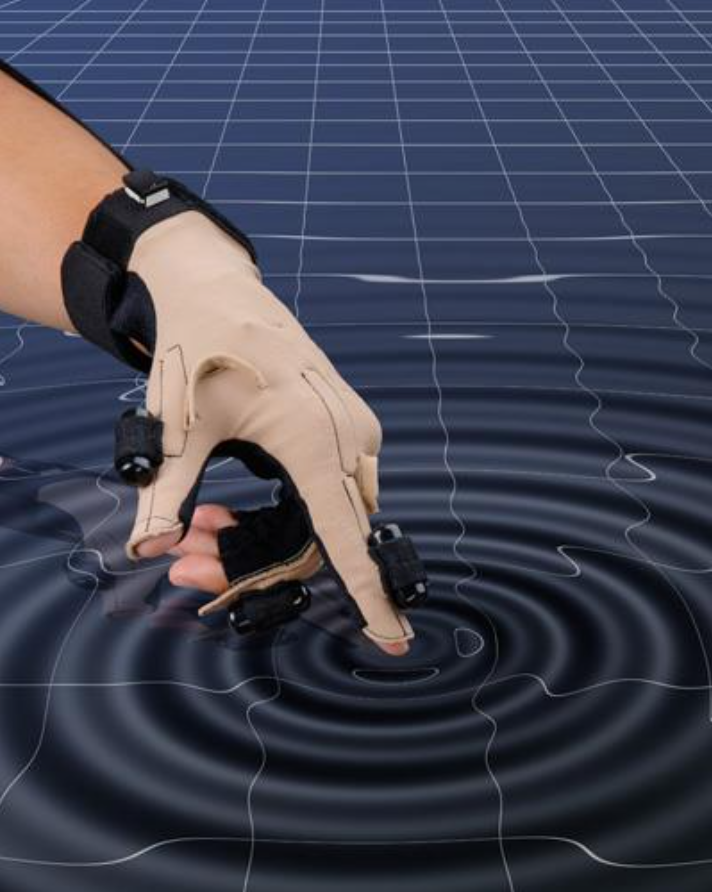
\includegraphics[width=\textwidth]{imgs/cybertouch}
\end{minipage}\\ 
\begin{minipage}[c]{0.65\textwidth}
\item CyberGrasp: Bisher ohne ForceFeedback! Daher wurde dieses Feature in dieser Entwicklungsstufe aufgegriffen. Mit diesem Gerät ist es möglich, virtuelle Objekte zu greifen. Man verspürt den Druck, den feste Gegenstände auf die eigene Hand ausüben. Die Art der Konstruktion des CyberGrasp bezeichnet man als exoskeletal, da die Kräfte mechanisch direkt auf das Skelett des Benutzers übertragen werden.
\end{minipage}\qquad
\begin{minipage}[c]{0.2\textwidth}
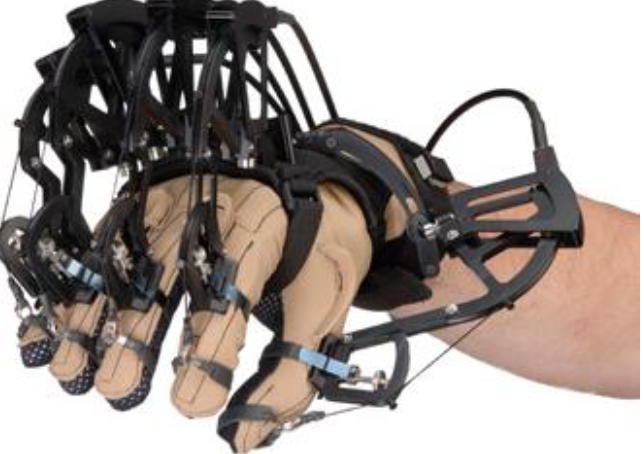
\includegraphics[width=\textwidth]{imgs/cybergrasp}
\end{minipage}\\ 
\begin{minipage}[c]{0.65\textwidth}
\item CyberForce: wieder eine Erweiterung der CyberGlove- und CyberGrasp-Technologie. Könnte man mit dem CyberGrasp nur Kräfte auf die Finger ausüben, so ist es mit diesem Gerät möglich, die ganze Hand zu lenken.
\end{minipage}\qquad
\begin{minipage}[c]{0.2\textwidth}
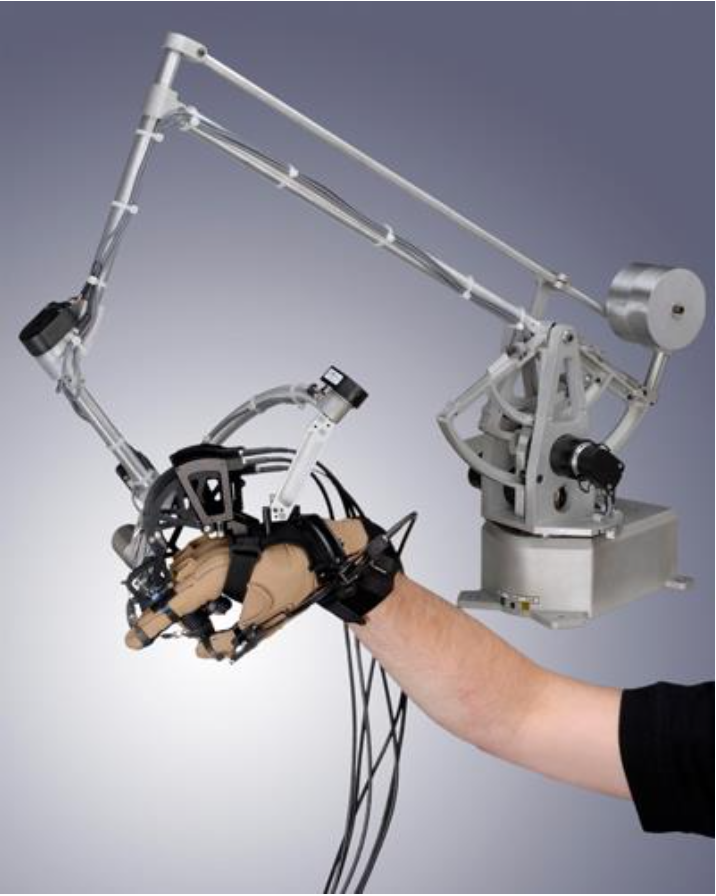
\includegraphics[width=\textwidth]{imgs/cyberforce}
\end{minipage}
\begin{minipage}[c]{0.65\textwidth}
\item BrainPort V100: Kamerabrille überträgt Schwarz-Weiß-Bilder an die Zunge, 20x20 Pixel Auflösung durch elektronische Stimulationsmuster, Ziel: Umgebung fühlen durch Kribbeln auf der Zunge, Erkennung: Umgebung, Position, Größe und Bewegung von Objekten
\end{minipage}\qquad
\begin{minipage}[c]{0.2\textwidth}
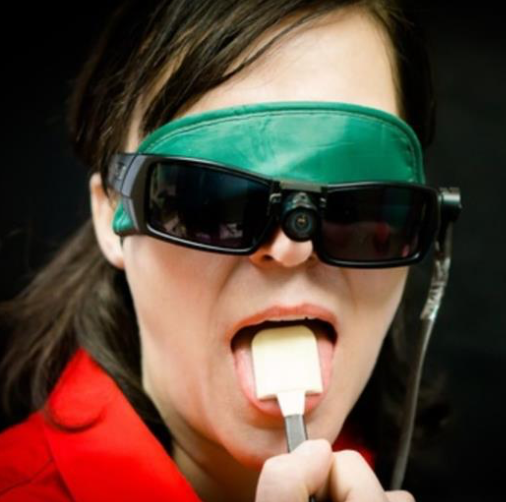
\includegraphics[width=\textwidth]{imgs/brainport}
\end{minipage}
\begin{minipage}[c]{0.65\textwidth}
\item Tacit Ultraschall Handsensor: 4 Ultraschallsensor, Abstandsmessung von 2cm bis 3,5cm, 2 Druck-Aktuatoren am Handrücken (für Hindernisse) links und rechts, Darstellung der Entfernung durch Druckstärke
\end{minipage}\qquad
\begin{minipage}[c]{0.2\textwidth}
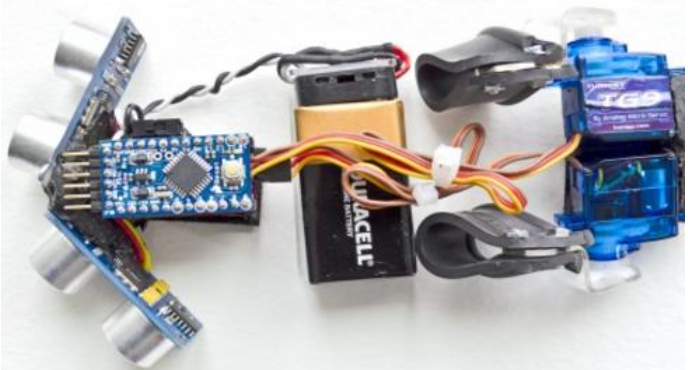
\includegraphics[width=\textwidth]{imgs/tacit}
\end{minipage}
\begin{minipage}[c]{0.65\textwidth}
\item Lechal Vibrationsschuhe: Haptischer Schuh mit GPS-basierter Navigation, Bluetooth-Schnittstelle zu Smartphone (App mit Sprachsteuerung), Vibration links oder rechts für Richtungsänderung, Ziel: Orientierung, Richtungsvorgabe, Hinderniserkennung, Gestiken (nach Hause navigieren, Position speichern, Notruf), Objekterkennung durch Sensoren im Schuh (Steine, Stufen, Schlaglöcher)
\end{minipage}\qquad
\begin{minipage}[c]{0.2\textwidth}
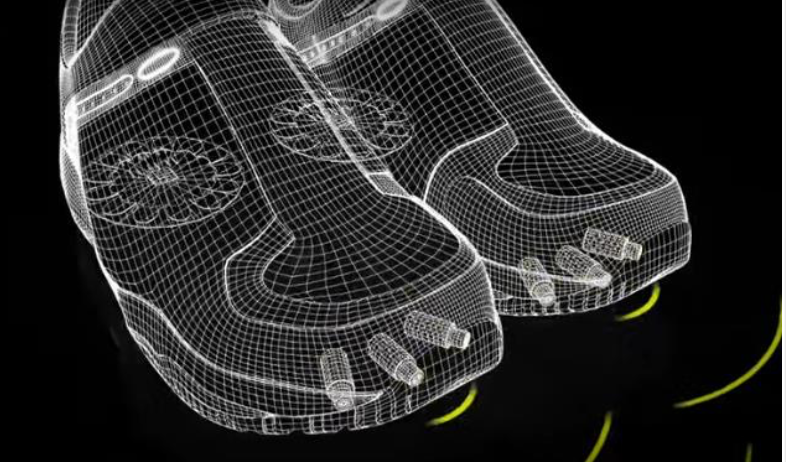
\includegraphics[width=\textwidth]{imgs/lechal}
\end{minipage}
\begin{minipage}[c]{0.65\textwidth}
\item Lechal Vibrationssohlen: Technik in die Schuhsohle integriert, keine Hinderniserkennung mehr, bis zu 15 Tage Akkulaufzeit, Preis 150 \$
\end{minipage}\qquad
\begin{minipage}[c]{0.2\textwidth}
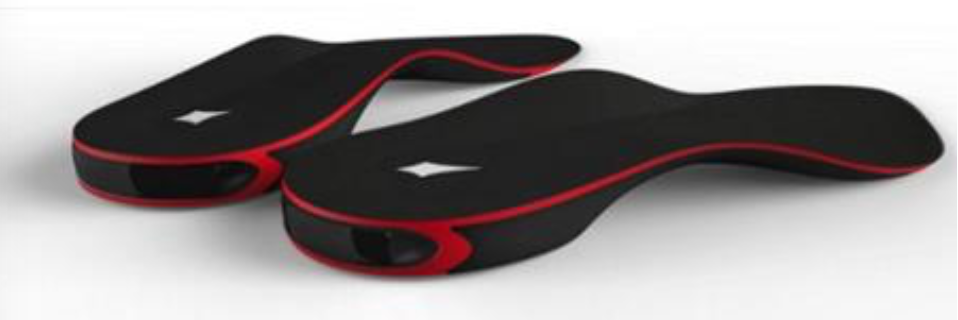
\includegraphics[width=\textwidth]{imgs/lechalsohlen}
\end{minipage}
\begin{minipage}[c]{0.65\textwidth}
\item Feelspace Gürtel: Vibrationsgürtel mit 3 Lithium-Ionen-Akkus, digitaler Kompass, 30 Vibrationsmotoren, 2 Kontroller (Signalverarbeitung + Stromversorgung)
\end{minipage}\qquad
\begin{minipage}[c]{0.2\textwidth}
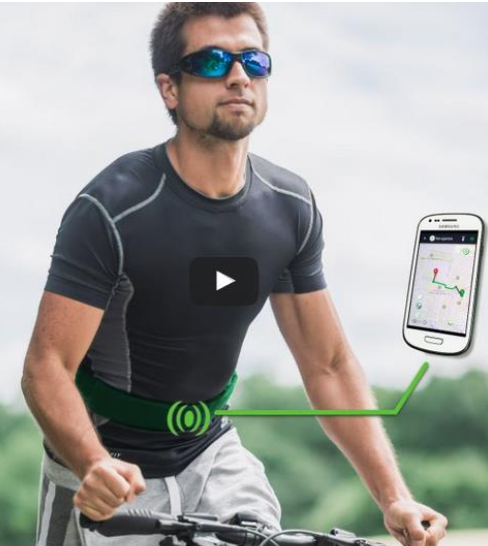
\includegraphics[width=\textwidth]{imgs/feelspace}
\end{minipage}
\begin{minipage}[c]{0.65\textwidth}
\item Dot: Braille Smartwatch für 300\$, Braille-Display zur Anzeige von Uhrzeit oder Handy-Nachrichten
\end{minipage}\qquad
\begin{minipage}[c]{0.2\textwidth}
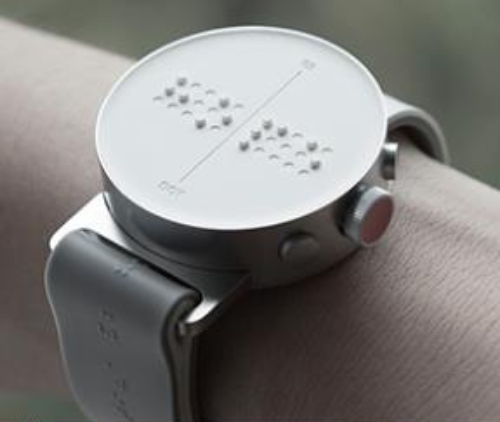
\includegraphics[width=\textwidth]{imgs/dot}
\end{minipage}
\end{itemize}
\end{itemize}

\subsection{Evaluierung}

\subsubsection{Grundlagen}

\begin{itemize}
\item Evaluierungen...
\begin{itemize}
\item sind ein wichtiger Bestandteil in allen Phasen einer Entwicklung
\item müssen mehrmals durchgeführt werden, damit eine gute Basis für zukünftige Entwicklungen bzw. Verbesserungen vorhanden ist
\item benötigen Zeit und Ressourcen. Daher bekommen sie häufig zu wenig Beachtung, worunter die Benutzerfreundlichkeit leidet.
\item sind wichtig, daher ist die richtige Evaluierungsmethode wichtig.
\end{itemize}
\item Evaluierungsgrundsätze
\begin{itemize}
\item Evaluierungen können zu verschiedenen Zeitpunkten oder aus verschiedenen Gründen durchgeführt werden
\item Es wird unterschieden, ob sie während eines Entwicklungsprozesses durchgeführt werden oder für bestehende Produkte
\end{itemize}
\item Beispiele für Evaluierungsmethoden
\begin{itemize}
\item Evaluierung durch Experten
\item Beobachtung der Nutzer
\item Interviews
\item Nachforschungen
\item lautes Denken
\item kognitives Durchgehen
\item Laborversuche zur Benutzerfreundlichkeit
\end{itemize}
\end{itemize}

\subsubsection{NASA-Task Load IndeX (TLX)}

\begin{itemize}
\item Gesamtpunktzahl (0-100, in 5er Schritten) aus 6 Bereichen:
\begin{itemize}
\item Geistige Anforderung: Wieviel geistige Wahrnehmungsaktivität war erforderlich? War die Aufgabe leicht oder anspruchsvoll, einfach oder komplex?
\item Physische Nachfrage: Wie viel körperliche Aktivität war erforderlich. War die aufgabe einfach oder anspruchsvoll, locker oder anstrengend?
\item Zeitliche Nachfrage: Fühlten Sie sich unter Zeitdruck durch das Tempo in dem die Vorgänge oder Aufgaben stattgefunden haben? War das Tempo zu langsam oder zu schnell?
\item Leistung: Wie erfolgreich waren Sie bei der Durchführung der Aufgabe? Wie zufrieden waren Sie mit Ihrer Leistung?
\item Aufwand: Wie sehr mussten Sie sich bemühen (geistig und körperlich), um Ihr Leistungsniveau zu erreichen?
\item Frust: Wie gereizt, gestresst und genervt fühlen Sie sich im Vergleich zu Inhalt bzw. wie entspannt und selbstzufrieden fühlt man sich während der Aufgabe?
\end{itemize}
\item kann als gültige und bewährte Metrik zur Auswertung von Benutzeroberflächen und Assistenzsystemen für blinde Anwendergruppen empfohlen werden
\item Blindgestellte sehende Nutzer sind keine gute Evaluationsgruppe
\item Idealerweise nur Blinde bzw. gemischte Testergruppen
\end{itemize}

\section{Computer Vision für Assistive Technologien}

Computer Vision für Blinde
\begin{itemize}
\item Color Processing: Erkennnung von Beleuchtung und Farben, Status von Geräten
\item 3D Stereo Vision: Hinderniserkennung, Bahnplanung
\item Objekterkennung: Erkennung/Wiederfinden von Gegenständen im Haushalt, Geldscheine, Medizin, Hinderniserkennung, Erkennung von Landmarken zur Orientierung, Anzeige zusätzlicher Information
\item Texterkennung: Handhabung von Geräten mit Text-Anzeige, Orientierung (Straßenschulder, Hausnummern, bestimmte Gebäude), Verkehrsschilder
\item Personenerkennung: Hinderniserkennung, reichhaltigere Wahrnehmung, Fingertracking zur Objektauswahl
\item High-Level Computer Vision: Erkennung von Handlungen, Situationen, Erzeugung sprachlicher Beschreibungen
\end{itemize}

\subsection{Hilfsmittel für den Alltag}

\begin{itemize}
\item Entwicklung eines tragbaren Assistenzsystems für Blinde
\begin{itemize}
\item Elektronischer Blindenhund, nur mächtiger
\item Hinderniserkennung
\item Personendetektion (Geschelcht, Alter, Identität)
\item Erkennung von Schildern und Text
\item Erkennung von Gebäuden (Navigation)
\item Objekterkennung
\item Interaktiv, mit Hand/Fingertracking (Klingeln, Objekte finden, ...)
\item Nutzung von GPS, Wifi, etc.
\end{itemize}
\item Ausgabe/Eingabe: Haptisch, akustisch, Text, Braille, ... (Benutzerstudien)
\item Sensorik und Computer können diskret in Kleidung eingearbeitet werden (wearable computing / intelligente Kleidung)
\item evtl. zusätzliche externe Kamerasensorik zu Hause (Wiederfinden von Objekten, Interaktion mit Umgebung)
\item Assistenzsystem zur Unterstützung der Mobilität
\begin{itemize}
\item Aufbau einer modularen Softwareplatform
\item Hindernis-/Freiflächenerkennung
\item Erkennung von Zebrastreifen, Straßenübergängen, Ampeln und Landmarken
\item Experimente zu audio-haptischen Schnittstellen
\end{itemize}
\item Object-Finder
\begin{itemize}
\item Suche nach eingelernten Objekten oder Farben
\item Ausgabe über 3D-Audio
\end{itemize}
\item Erkennung von Straßenbahntüren
\item Benutzerstudien und Umfragen
\end{itemize}

\subsection{Wie funktioniert Bildverarbeitung?}

\begin{itemize}
\item Automatische Analyse von Bildern und Videos
\item Teilgebiet der Mustererkennung
\item Teilgebiet der Künstlichen Intelligenz
\item Teilgebiet der Informatik (und Elektrotechnik)
\item Analyse von vielen Pixeln
\end{itemize}

\subsection{Objekt-/Gebäude-/Texterkennung}

\begin{itemize}
\item Objekterkennung
\begin{itemize}
\item Sehr aktives Forschungsgebiet, große Fortschritte, zahlreiche Benchmarks
\item $\approx$ 30\% Fehler bei 256 Klassen (Caltech-Benchmark)
\item Deutlich höhere Erkennungsrate für spezifische Objekte: Meine Kaffeetasse, bestimmte Gegenstände, Nahrungsmittel, Verpackungen, Erkennung von Geldscheinen
\item Assistenzgerät könnte Name des angefassten Objekts sprechen
\end{itemize}
\item Erkennung von Gebäuden/Landmarken
\begin{itemize}
\item Erkennung von Gebäuden und Orten (Gebäudeansichten können wie Objekte eintrainiert werden)
\item Nutzung von Bilddatenbank im Web zum automatischen Aufbau von Landmarken-Detektoren
\item Hilfreich zur Orientierung, Finden bestimmter Gebäude
\item Ansage zusätzlicher Informationen
\end{itemize}
\item Erkennung von Schildern und Text
\begin{itemize}
\item Erkennung von Verkehrsschildern in Fahrzeugen bereits erhältlich
\item Detektion und Erkennung von Text (verschiedene Forschungsarbeiten, Detektion von Text, dann OCR)
\item Anwendungen: Orientierung (Straßennamen, Geschäfte, Hausnummern), Finden von Namensschildern, Sicherheit (Verkehrsschilder), Benutzung von Geräten: Lesen von LED Anzeigen
\end{itemize}
\item Erzeugung Textlicher Beschreibungen
\begin{itemize}
\item Ziel: Interpretation der Bild- / Videoinhalte
\item Erzeugung von natürlichsprachlichen Beschreibungen
\item Zahlreiche Forschungsarbeiten: Verkehrsszenen, Spiele, Sport, menschliche Interaktion, Smart Rooms, Automatische Annotation von Bildern
\end{itemize}
\end{itemize}

\subsection{ImageNet}

\begin{itemize}
\item Aufgabe: Objekterkennung mit 1000 Klassen und 1,3 Millionen gelabelten Trainingsdaten
\item Bestes Top-5 Ergebnis derzeit unter 4\%
\end{itemize}

\subsection{Personenerkennung}

\begin{itemize}
\item Zahlreiche Forschungsarbeiten zur Personendetektion und -Tracking: Große Fortschritte, 3D Multipersonentracking in Echtzeit möglich, erste Detektionssysteme im Automobilbereich
\item Identifikation, Alterus- und Geschlechts-, Mimik-, Handlungserkennung möglich
\item Anwendungen: Kollisionsvermeidung, Erkennung der Lauf- und Blickrichtung, Unterstützung der Kommunikation (wer schaut wen an, Mimik, Zeigegesten), Identikation (Zuganssysteme, personalisierte Dienste)
\end{itemize}

\section{Smarthome}

\subsection{Definition}

\begin{itemize}
\item Als Smart Home bezeichnet man einen Haushalt, in dem Haushalts- und Multimedia-Geräte interagieren und zentral ferngesteuert werden können
\item Automatisierung von Alltagsvorgängen
\item Schnelle und flexible Anpassung von verschiedenen Geräten an persönliche Bedürfnisse
\item Smart Home als neue Generation der Hausautomation ermöglicht durch bidirektionale Funkstandards (WLAN/Blutetooth) und Smartphones oder Tablets als Fernbedienung.
\item Jedes Smart Home System hat ein Herzstück: Die Smart Home Zentrale (mit dieser werden smarte Geräte verbunden und per Computer, Smartphone oder Tablet gesteuert, jede Zentrale spricht eine oder mehrere (Funk-)Sprachen, darunter KNX, WLAN, Bluetooth, ZigBee, Z-Wave)
\end{itemize}

\subsection{Barrierefreie Features im Haus}

\begin{itemize}
\item Elektrische Fenster und Rollläden (automatisch gesteuert)
\item Beleuchtung mit intelligenten Bewegungs- und Präsenzmeldern (Sicherheit)
\item Morderne Türen mit Türsprechanlage/Motorschloss (Sicherheit+Komfort)
\item Schalter und Steckdosen barrierefrei platzieren (ideal sind 85cm für Schalter und 40cm für Steckdosen)
\item Sonstige Features: Smartphone-Integration, Alarmanlage, Fenster/Tür-Überwachung, Musik über Präsenzmelder, Rauchmelder, Wassersensoren, Bewässerung, Multiroom-Soundsysteme (z.B. Sonos, Telefonmeldung, Haustür, automatisches Pausieren)
\end{itemize}

\subsection{Bus-Systeme}

\begin{itemize}
\item Europäischer Installationsbus (EIB) ist ein Standard nach EN 50090, in der aktuellen Version als \textbf{KNX}-Standard auch nach ISO/IEC 14543-3: beschreibt wie bei einer Installation Sensoren und Aktoren in einem Haus miteinander verbinden werden können, legt fest wie Sensoren und Aktoren miteinander kommunizieren müssen
\item KNX: Nachfolger der Feldbusse EIB, BatiBus und EHS, technisch eine Weiterentwicklung des EIB durch Erweiterung um Konfigurationsmechanismen und Übertragungsmedien, die ursprünglich für BatiBus und EHS entwickelt wurden, mit EIB kompatibel
\item ZigBee Pro: verwendet bei Lightify, Miele, Philips Hue, Qivicon, wibutler
\item Z-Wave: verwendet bei Devolo, wibutler, Fibaro, EWE Vetrieb GmbH
\item Enocean: verwendet von vielen Herstellern
\item HomeMatic: verwendet von Qivicon und RWE
\item WLAN: Apple HomeKit, wibutler, TP-Link
\item io-homecontrol: Somfy, Velux
\item DECT ULE: Panasonic, Gigaset Elements, AVM
\item 1-Wire: Sensorik
\end{itemize}

\section{Aktuelle Forschung}

\begin{itemize}
\item Cooperate: Entwicklung und Evaluierung eines modellhaften UML-Kooperationswerkzeugs für Diversity Teams in der Softwareentwicklung, Entwurf eines Schulungskonzeptes für Präsenzveranstaltungen und das Selbststudium, Entwicklung eines Leitfadens für barrierefreie Kooperationswerkzeuge in der Softwareentwicklung
\item Terrain: Selbstständige Mobilität blinder und sehbehinderter Menschem im urbanen Raum durch audio-taktile Navigation
\item AT-Maps: Spezifikationen von Symbolen für audio-taktile Karten für Menschen mit Blindheit
\item Learning PDF document structure for Accessibility: Dokumentenstruktur verstehen und erkennen, automatisches taggen digital erstellter PDFs, erlernen von Dokumentenstrukturen aus getaggten Dokumenten, Neu-Setzen der Informationen $\rightarrow$ barrierefreie PDF
\item TPad - SZS: Audio-taktiler Grafikzugang für Blinde mit Standard-Komponenten
\item VR für Sehbehinderte: beliebige Größe der Inhalte, Kontrast, Helligkeit, Farbtöne an Benutzer anpassbar, verbesserte Darstellung $\rightarrow$ einfachere Arbeit am PC mit Sehbehinderung
\end{itemize}

\end{document}